\documentclass{beamer} 

\usepackage{hayesmacros}
\usepackage{appendixnumberbeamer}

\usetheme{metropolis}
\setsansfont{Fira Sans}  % be sure to compile with XeLaTeX

\usepackage{natbib}
\usepackage{ulem}
\usepackage{fontawesome5}
\usepackage{twemojis}

\newtheorem{proposition}{Proposition}
\newtheorem{assumption}{Assumption}

\theoremstyle{remark}
\newtheorem*{remark}{Remark}

\setbeamercolor{background canvas}{bg=white}
\setbeamercolor{normal text}{fg=black}
\setbeamercolor{frametitle}{bg=black, fg=white}

\hypersetup{colorlinks,citecolor=cyan, urlcolor=cyan, linkcolor=black}

\title{Estimating network-mediated causal effects via spectral embeddings}
\date{2023-03-24 @ IFDS Ideas Forum \\ Department of Statistics, University of Wisconsin-Madison}
\author{Alex Hayes}
\institute{Slides available at \url{https://tinyurl.com/ifds-alex}}


\begin{document}

\maketitle

\begin{frame}{This is joint work!}

    \begin{columns}
        \centering

        \column{0.5 \textwidth}

        \begin{figure}
            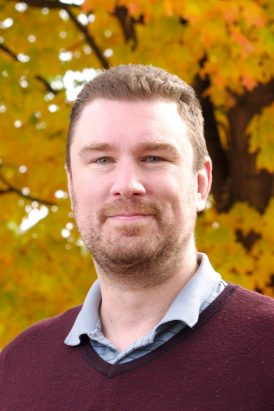
\includegraphics[width=4cm]{figures/mark.jpg}
        \end{figure}

        \centering

        Mark Fredrickson

        University of Michigan

        \column{0.5 \textwidth}
        \centering

        \begin{figure}
            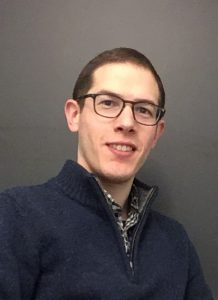
\includegraphics[width=4cm]{figures/keith.jpg}
        \end{figure}

        Keith Levin

        UW-Madison

    \end{columns}

\end{frame}


\begin{frame}{Two questions for the audience}

    1. How familiar are you with directed acyclic graphs?


    2. How familiar are you with stochastic block models?

\end{frame}


\begin{frame}{A short story about arriving in Madison \& the Great Dane}

    \begin{center}
        \begin{tikzpicture}
            \node (me) at (0,6) {\Huge \texttwemoji{man standing}};

            \node (f1) at (1,6) {};
            \node (f2) at (1,5) {};
            \node (f3) at (0.5,5.5) {};
            \node (f4) at (0,5) {};
            \node (f5) at (-0.5,5.5) {};

            \node (g1) at (3,6) {};
            \node (g2) at (3,5) {};
            \node (g3) at (2.5,5.5) {};
            \node (g4) at (2,5) {};
            \node (g5) at (3.5,5.5) {};

            \node (h1) at (1,1) {};
            \node (h2) at (1,0) {};
            \node (h3) at (0.5,0.5) {};
            \node (h4) at (0,0) {};
            \node (h5) at (-0.5,0.5) {};

            \node (i1) at (6,0) {};
            \node (i2) at (5,1) {};
            \node (i3) at (5.5,0.5) {};
            \node (i4) at (5,0) {};

        \end{tikzpicture}
    \end{center}

\end{frame}

\begin{frame}{I didn't know anyone when I first arrived here}

    \begin{center}
        \begin{tikzpicture}
            \node (me) at (0,6) {\Huge \texttwemoji{man standing}};

            \node (f1) at (1,6) {\Huge \texttwemoji{person standing}};
            \node (f2) at (1,5) {\Huge \texttwemoji{person standing}};
            \node (f3) at (0.5,5.5) {\Huge \texttwemoji{person standing}};
            \node (f4) at (0,5) {\Huge \texttwemoji{person standing}};
            \node (f5) at (-0.5,5.5) {\Huge \texttwemoji{person standing}};

            \node (g1) at (3,6) {\Huge \texttwemoji{person standing}};
            \node (g2) at (3,5) {\Huge \texttwemoji{person standing}};
            \node (g3) at (2.5,5.5) {\Huge \texttwemoji{person standing}};
            \node (g4) at (2,5) {\Huge \texttwemoji{person standing}};
            \node (g5) at (3.5,5.5) {\Huge \texttwemoji{person standing}};

            \node (h1) at (1,1) {\Huge \texttwemoji{person standing}};
            \node (h2) at (1,0) {\Huge \texttwemoji{person standing}};
            \node (h3) at (0.5,0.5) {\Huge \texttwemoji{person standing}};
            \node (h4) at (0,0) {\Huge \texttwemoji{person standing}};
            \node (h5) at (-0.5,0.5) {\Huge \texttwemoji{person standing}};

            \node (i1) at (6,0) {\Huge \texttwemoji{person standing}};
            \node (i2) at (5,1) {\Huge \texttwemoji{person standing}};
            \node (i3) at (5.5,0.5) {\Huge \texttwemoji{person standing}};
            \node (i4) at (5,0) {\Huge \texttwemoji{person standing}};

        \end{tikzpicture}
    \end{center}

\end{frame}

\begin{frame}{But! I like frisbee, so I joined a frisbee team!}

    \begin{center}
        \begin{tikzpicture}
            \node (me) at (0,6) {\Huge \texttwemoji{man playing handball}};

            \node (f1) at (1,6) {\Huge \texttwemoji{person playing handball}};
            \node (f2) at (1,5) {\Huge \texttwemoji{person playing handball}};
            \node (f3) at (0.5,5.5) {\Huge \texttwemoji{person playing handball}};
            \node (f4) at (0,5) {\Huge \texttwemoji{person playing handball}};
            \node (f5) at (-0.5,5.5) {\Huge \texttwemoji{person playing handball}};

            \node (g1) at (3,6) {\Huge \texttwemoji{person standing}};
            \node (g2) at (3,5) {\Huge \texttwemoji{person standing}};
            \node (g3) at (2.5,5.5) {\Huge \texttwemoji{person standing}};
            \node (g4) at (2,5) {\Huge \texttwemoji{person standing}};
            \node (g5) at (3.5,5.5) {\Huge \texttwemoji{person standing}};

            \node (h1) at (1,1) {\Huge \texttwemoji{person standing}};
            \node (h2) at (1,0) {\Huge \texttwemoji{person standing}};
            \node (h3) at (0.5,0.5) {\Huge \texttwemoji{person standing}};
            \node (h4) at (0,0) {\Huge \texttwemoji{person standing}};
            \node (h5) at (-0.5,0.5) {\Huge \texttwemoji{person standing}};

            \node (i1) at (6,0) {\Huge \texttwemoji{person standing}};
            \node (i2) at (5,1) {\Huge \texttwemoji{person standing}};
            \node (i3) at (5.5,0.5) {\Huge \texttwemoji{person standing}};
            \node (i4) at (5,0) {\Huge \texttwemoji{person standing}};

            \draw (me) -- (f3);
            \draw (f1) -- (f3);
            \draw (f2) -- (f3);
            \draw (f4) -- (f3);
            \draw (f4) -- (f5);
            \draw (f4) -- (f1);
            \draw (me) -- (f5);
            \draw (me) -- (f1);

        \end{tikzpicture}
    \end{center}

\end{frame}

\begin{frame}{The Madison social network}

    \begin{center}
        \begin{tikzpicture}
            \node (me) at (0,6) {\Huge \texttwemoji{man playing handball}};

            \node (f1) at (1,6) {\Huge \texttwemoji{person playing handball}};
            \node (f2) at (1,5) {\Huge \texttwemoji{person playing handball}};
            \node (f3) at (0.5,5.5) {\Huge \texttwemoji{person playing handball}};
            \node (f4) at (0,5) {\Huge \texttwemoji{person playing handball}};
            \node (f5) at (-0.5,5.5) {\Huge \texttwemoji{person playing handball}};

            \node (g1) at (3,6) {\Huge \texttwemoji{person rowing boat}};
            \node (g2) at (3,5) {\Huge \texttwemoji{person rowing boat}};
            \node (g3) at (2.5,5.5) {\Huge \texttwemoji{person rowing boat}};
            \node (g4) at (2,5) {\Huge \texttwemoji{person rowing boat}};
            \node (g5) at (3.5,5.5) {\Huge \texttwemoji{person rowing boat}};

            \node (h1) at (1,1) {\Huge \texttwemoji{person climbing}};
            \node (h2) at (1,0) {\Huge \texttwemoji{person climbing}};
            \node (h3) at (0.5,0.5) {\Huge \texttwemoji{person climbing}};
            \node (h4) at (0,0) {\Huge \texttwemoji{person climbing}};
            \node (h5) at (-0.5,0.5) {\Huge \texttwemoji{person climbing}};

            \node (i1) at (6,0) {\Huge \texttwemoji{person fencing}};
            \node (i2) at (5,1) {\Huge \texttwemoji{person fencing}};
            \node (i3) at (5.5,0.5) {\Huge \texttwemoji{person fencing}};
            \node (i4) at (5,0) {\Huge \texttwemoji{person fencing}};

            \draw (me) -- (f3);
            \draw (f1) -- (f3);
            \draw (f2) -- (f3);
            \draw (f4) -- (f3);
            \draw (f4) -- (f5);
            \draw (f4) -- (f1);
            \draw (me) -- (f5);
            \draw (me) -- (f1);

            \draw (g1) -- (g3);
            \draw (g2) -- (g3);
            \draw (g4) -- (g3);
            \draw (g4) -- (g5);
            \draw (g4) -- (g1);
            \draw (g2) -- (g5);
            \draw (g4) -- (g1);

            \draw (h1) -- (h3);
            \draw (h2) -- (h3);
            \draw (h4) -- (h3);
            \draw (h4) -- (h5);
            \draw (h4) -- (h1);
            \draw (h2) -- (h5);
            \draw (h4) -- (h1);

            \draw (i1) -- (i3);
            \draw (i2) -- (i3);
            \draw (i4) -- (i3);
            \draw (i4) -- (i1);
            \draw (i4) -- (i2);

            \draw (h4) -- (g1);
            \draw (h2) -- (g5);
            \draw (f4) -- (h1);
            \draw (i1) -- (f3);
            \draw (g2) -- (i3);
            \draw (h2) -- (i3);
            \draw (g2) -- (f3);

        \end{tikzpicture}
    \end{center}

\end{frame}


\begin{frame}{Madison frisbee players go the Great Dane fairly often!}

    \begin{center}
        \begin{tikzpicture}
            \node (me) at (0,6) {\Huge \texttwemoji{man playing handball}};

            \node (f1) at (1,6) {\Huge \texttwemoji{person playing handball}};
            \node (f2) at (1,5) {\Huge \texttwemoji{person playing handball}};
            \node (f3) at (0.5,5.5) {\Huge \texttwemoji{person playing handball}};
            \node (f4) at (0,5) {\Huge \texttwemoji{person playing handball}};
            \node (f5) at (-0.5,5.5) {\Huge \texttwemoji{person playing handball}};

            \node (g1) at (3,6) {\Huge \texttwemoji{person rowing boat}};
            \node (g2) at (3,5) {\Huge \texttwemoji{person rowing boat}};
            \node (g3) at (2.5,5.5) {\Huge \texttwemoji{person rowing boat}};
            \node (g4) at (2,5) {\Huge \texttwemoji{person rowing boat}};
            \node (g5) at (3.5,5.5) {\Huge \texttwemoji{person rowing boat}};

            \node (h1) at (1,1) {\Huge \texttwemoji{person climbing}};
            \node (h2) at (1,0) {\Huge \texttwemoji{person climbing}};
            \node (h3) at (0.5,0.5) {\Huge \texttwemoji{person climbing}};
            \node (h4) at (0,0) {\Huge \texttwemoji{person climbing}};
            \node (h5) at (-0.5,0.5) {\Huge \texttwemoji{person climbing}};

            \node (i1) at (6,0) {\Huge \texttwemoji{person fencing}};
            \node (i2) at (5,1) {\Huge \texttwemoji{person fencing}};
            \node (i3) at (5.5,0.5) {\Huge \texttwemoji{person fencing}};
            \node (i4) at (5,0) {\Huge \texttwemoji{person fencing}};

            \node (house) at (-1.3, 5) {\Huge \texttwemoji{house with garden}};
            \node (house) at (-2, 4.5) {\Huge \texttwemoji{beers}};
            \node (house) at (-1.9, 5.5) {\Huge \texttwemoji{hamburger}};

            \draw (me) -- (f3);
            \draw (f1) -- (f3);
            \draw (f2) -- (f3);
            \draw (f4) -- (f3);
            \draw (f4) -- (f5);
            \draw (f4) -- (f1);
            \draw (me) -- (f5);
            \draw (me) -- (f1);

            \draw (g1) -- (g3);
            \draw (g2) -- (g3);
            \draw (g4) -- (g3);
            \draw (g4) -- (g5);
            \draw (g4) -- (g1);
            \draw (g2) -- (g5);
            \draw (g4) -- (g1);

            \draw (h1) -- (h3);
            \draw (h2) -- (h3);
            \draw (h4) -- (h3);
            \draw (h4) -- (h5);
            \draw (h4) -- (h1);
            \draw (h2) -- (h5);
            \draw (h4) -- (h1);

            \draw (i1) -- (i3);
            \draw (i2) -- (i3);
            \draw (i4) -- (i3);
            \draw (i4) -- (i1);
            \draw (i4) -- (i2);

            \draw (h4) -- (g1);
            \draw (h2) -- (g5);
            \draw (f4) -- (h1);
            \draw (i1) -- (f3);
            \draw (g2) -- (i3);
            \draw (h2) -- (i3);
            \draw (g2) -- (f3);

        \end{tikzpicture}
    \end{center}

\end{frame}

\section{Idea: social groups \emph{mediate} the causal effect of individual interests (e.g. frisbee) on visits to the Great Dane}

\begin{frame}{I like frisbee ($T_i$) so I join a frisbee team ($\X_{i \cdot}$)}

    \centering

    \begin{figure}
        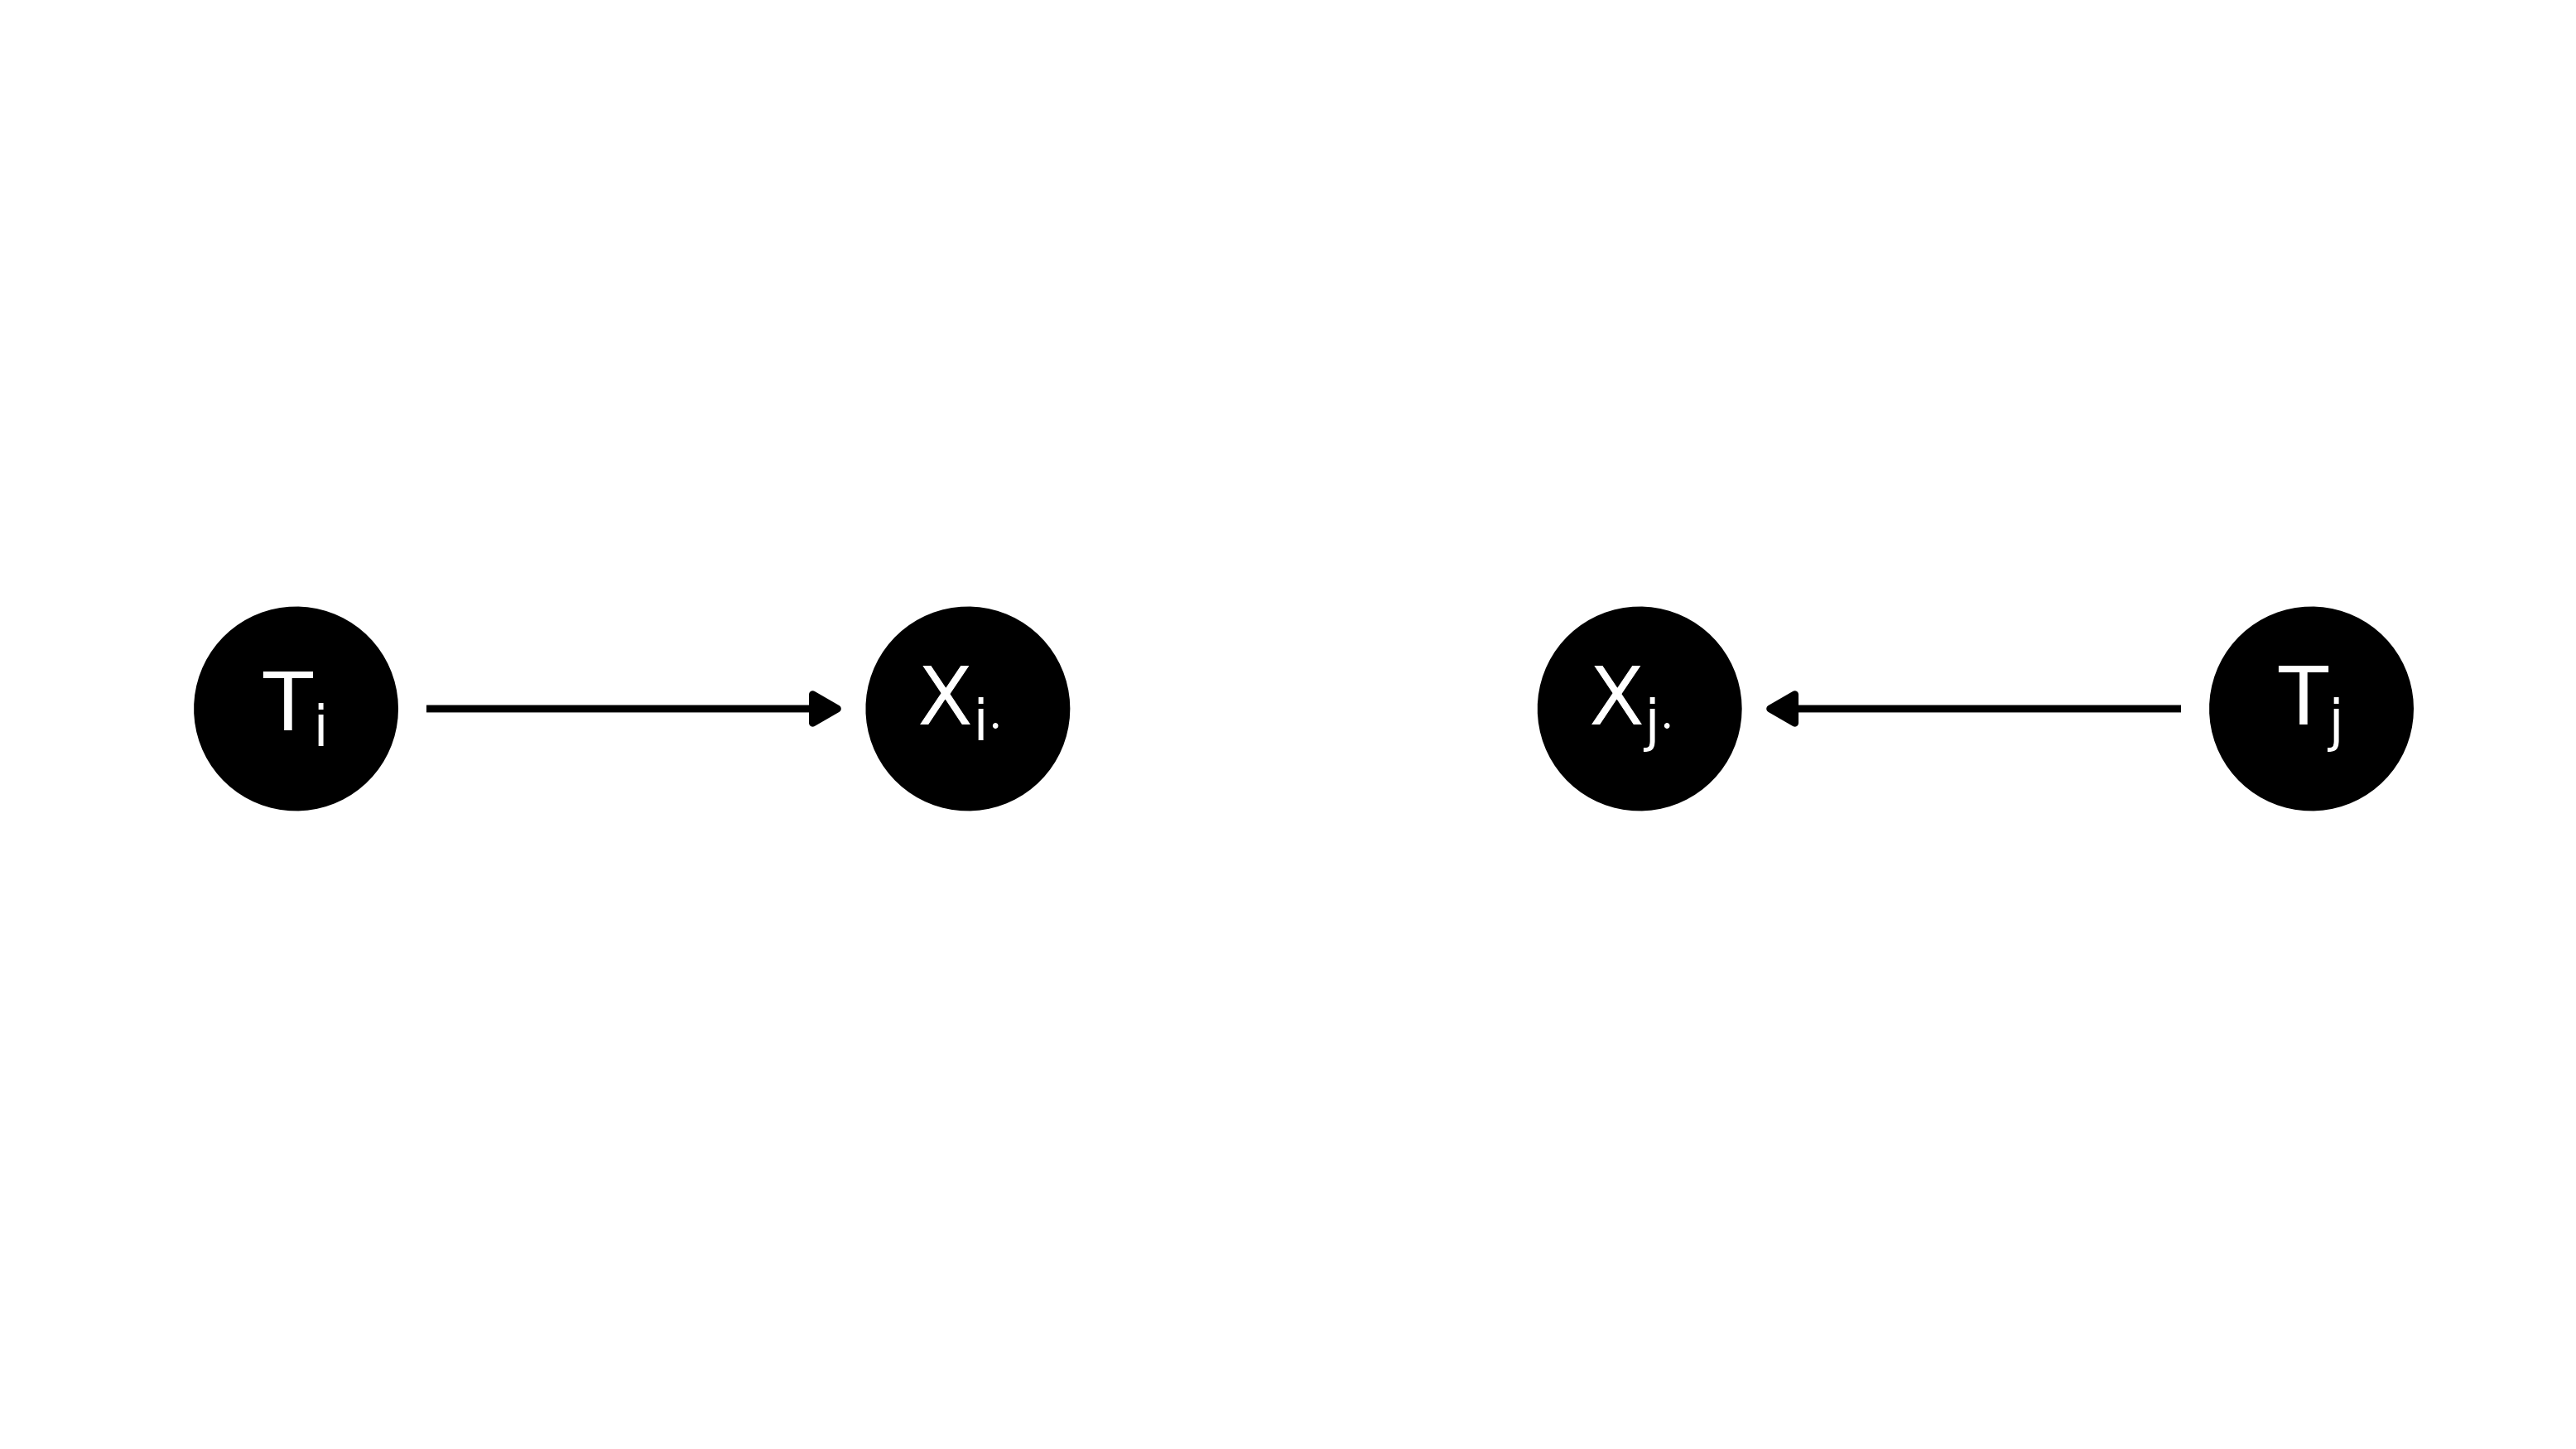
\includegraphics[scale=0.65]{figures/dags/mediating-1.png}
        \label{fig:mediating-1}
    \end{figure}

    Assume there are only two people, person $i$ and person $j$

\end{frame}

\begin{frame}{I'm on a frisbee team, so I form friendships ($A_{ij}$) with other people on my team}

    \centering

    \begin{figure}
        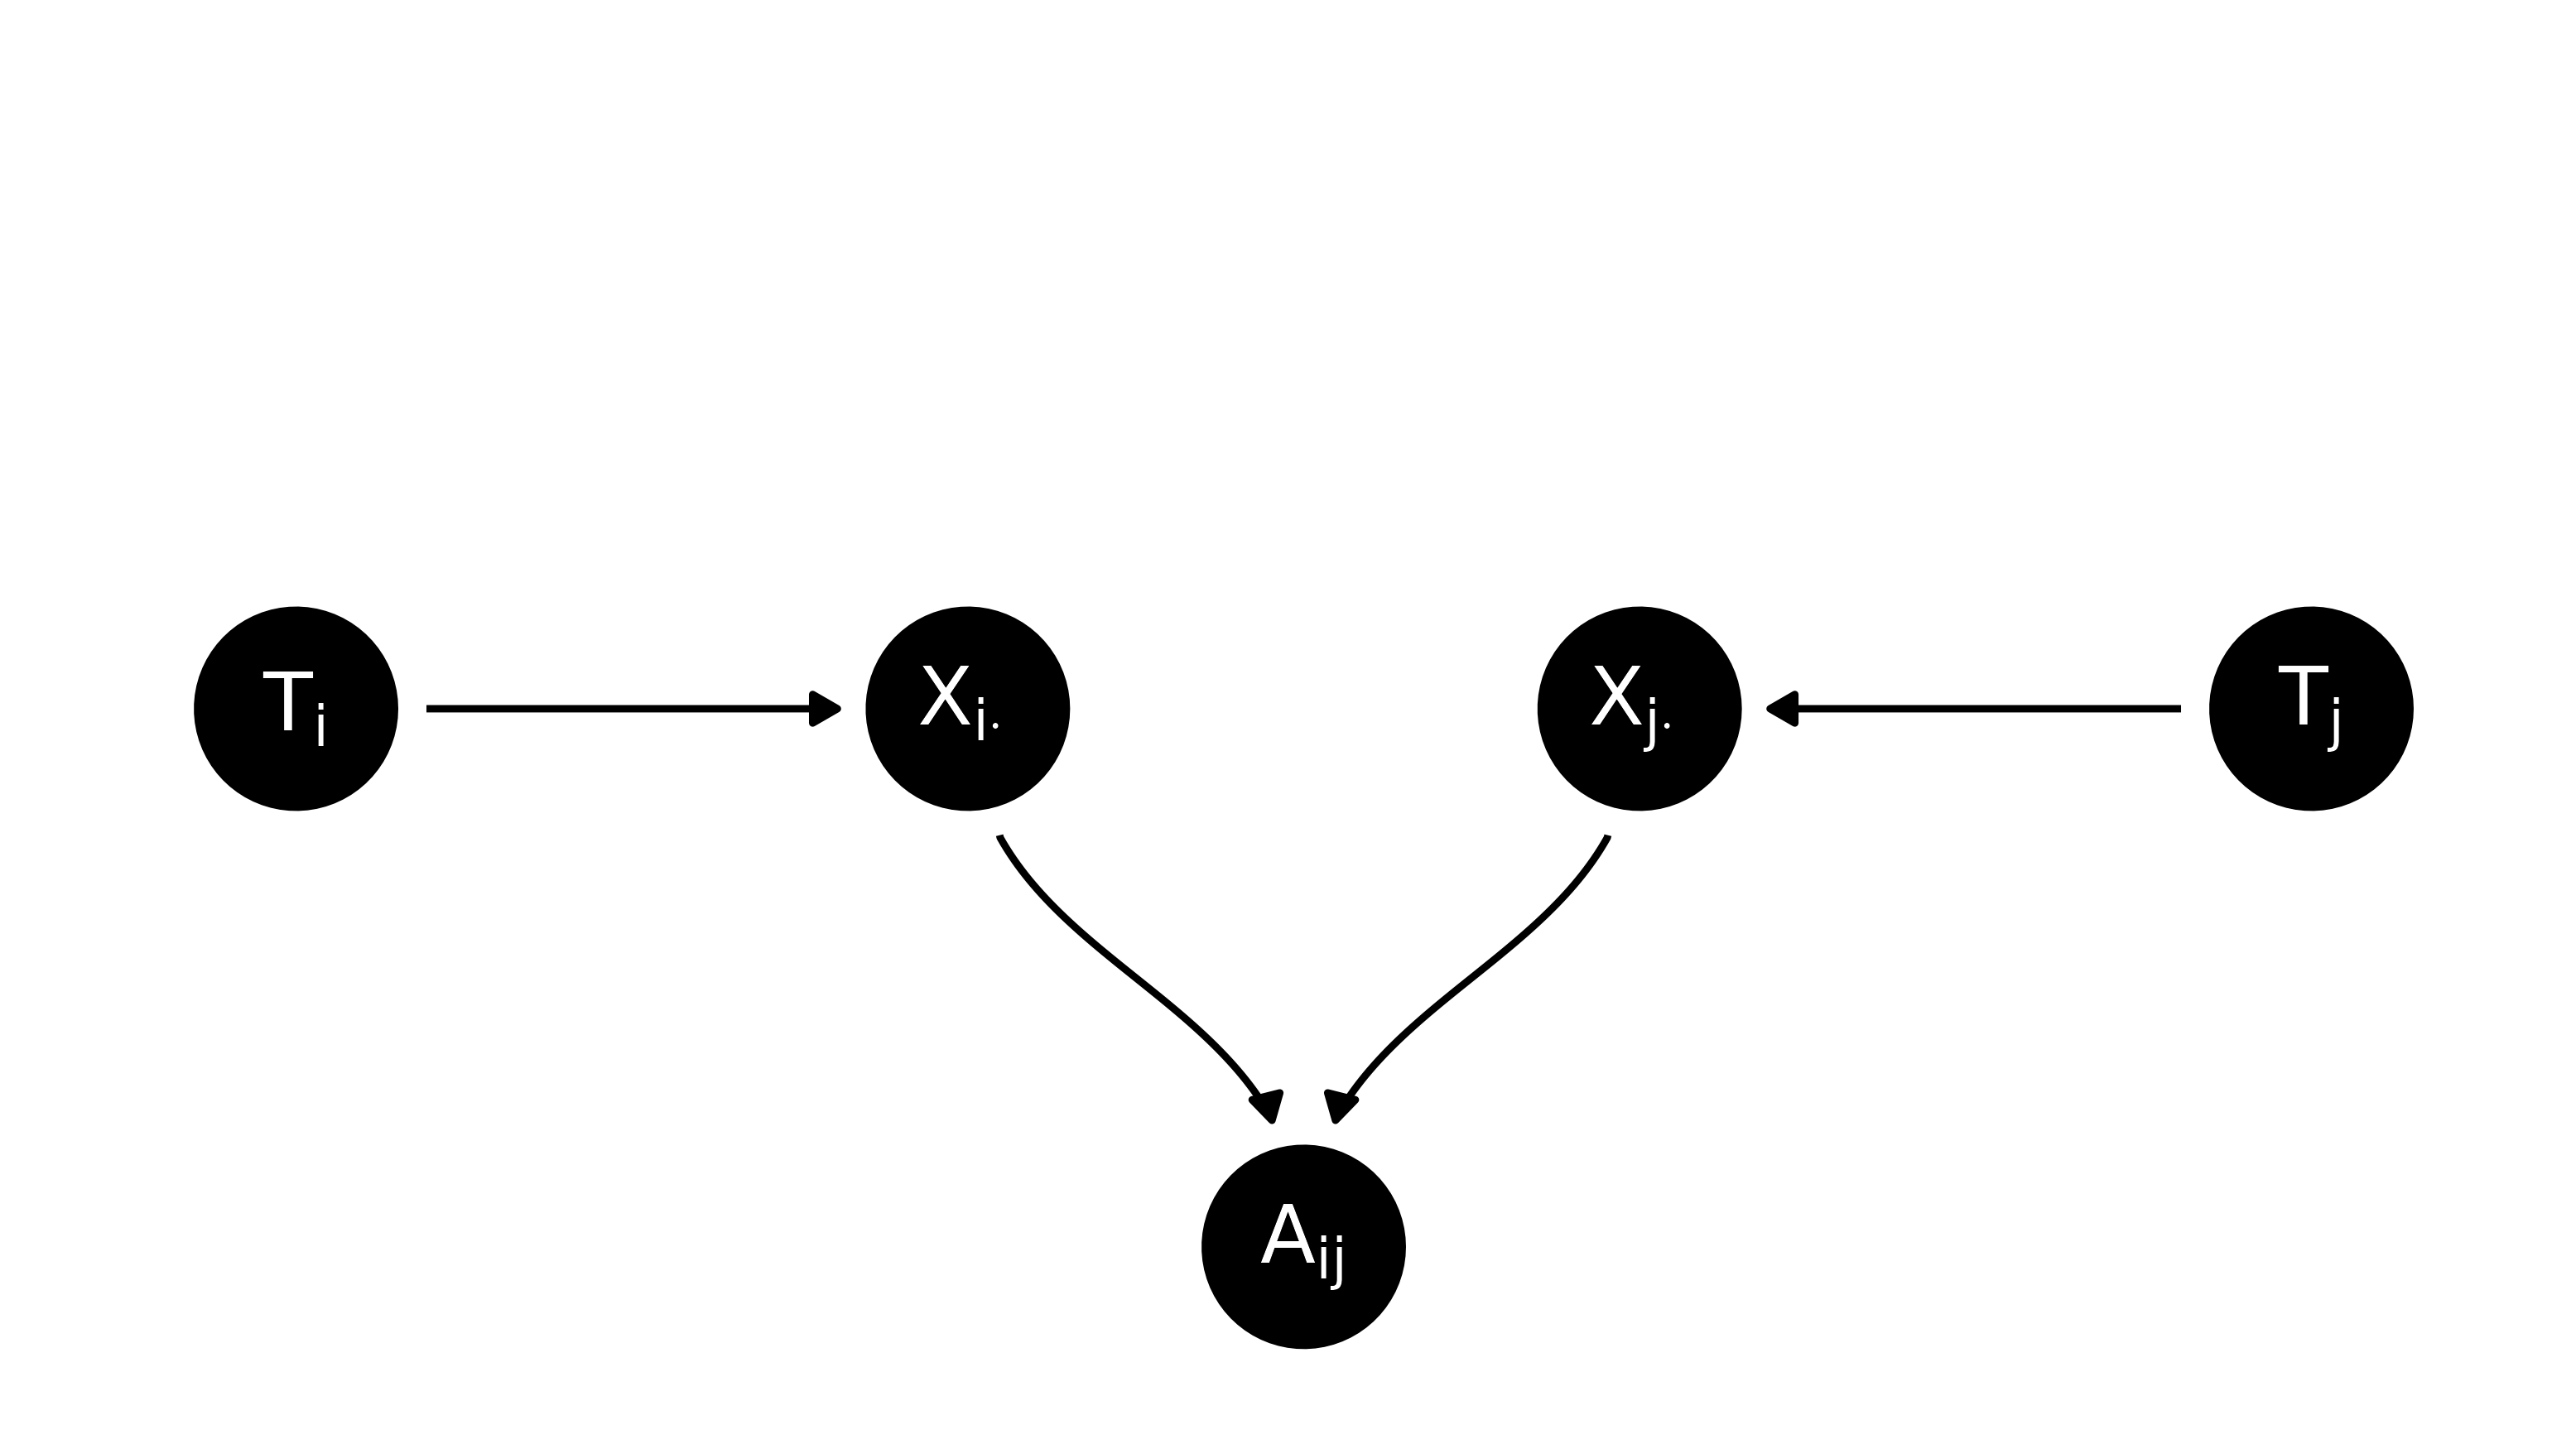
\includegraphics[scale=0.65]{figures/dags/mediating-2.png}
        \label{fig:mediating-2}
    \end{figure}

\end{frame}

\begin{frame}{I'm on a frisbee team, so I go to the Great Dane ($Y_i$)}

    \centering

    \begin{figure}
        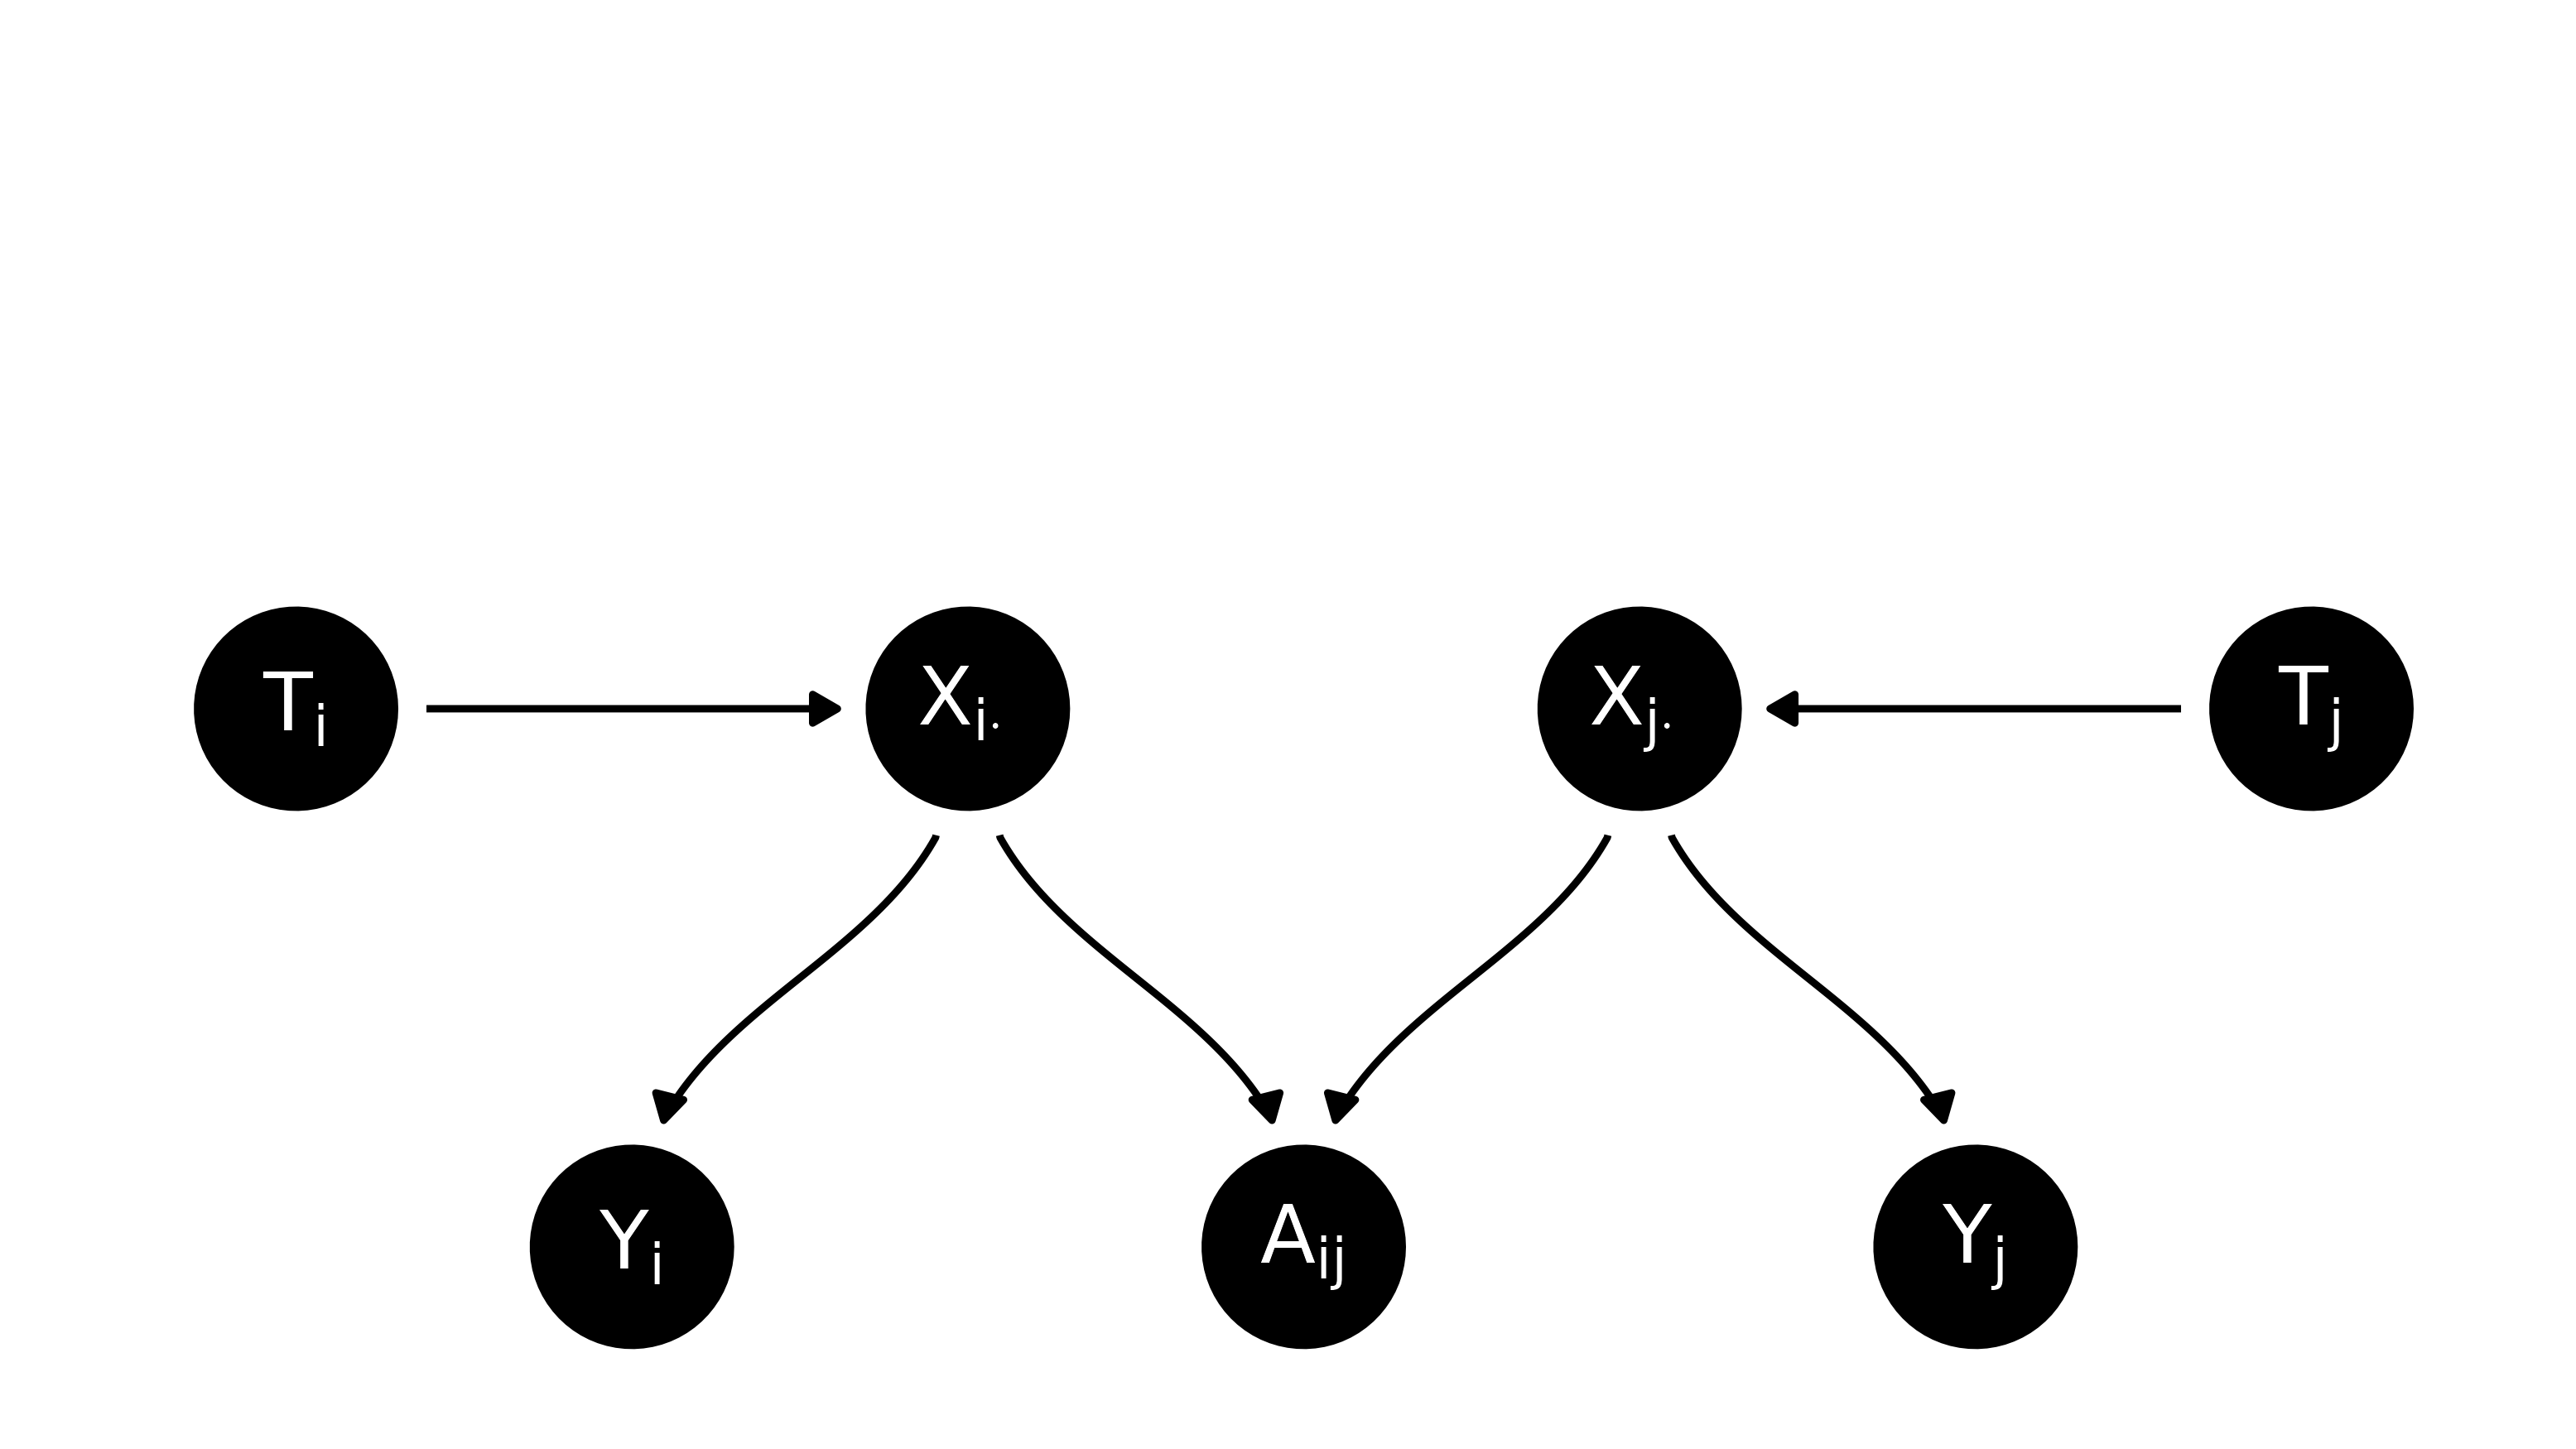
\includegraphics[scale=0.65]{figures/dags/mediating-3.png}
        \label{fig:mediating-3}
    \end{figure}

\end{frame}

\begin{frame}{I like frisbee, and this might directly cause me to go to the Great Dane without my team}

    \centering

    \begin{figure}
        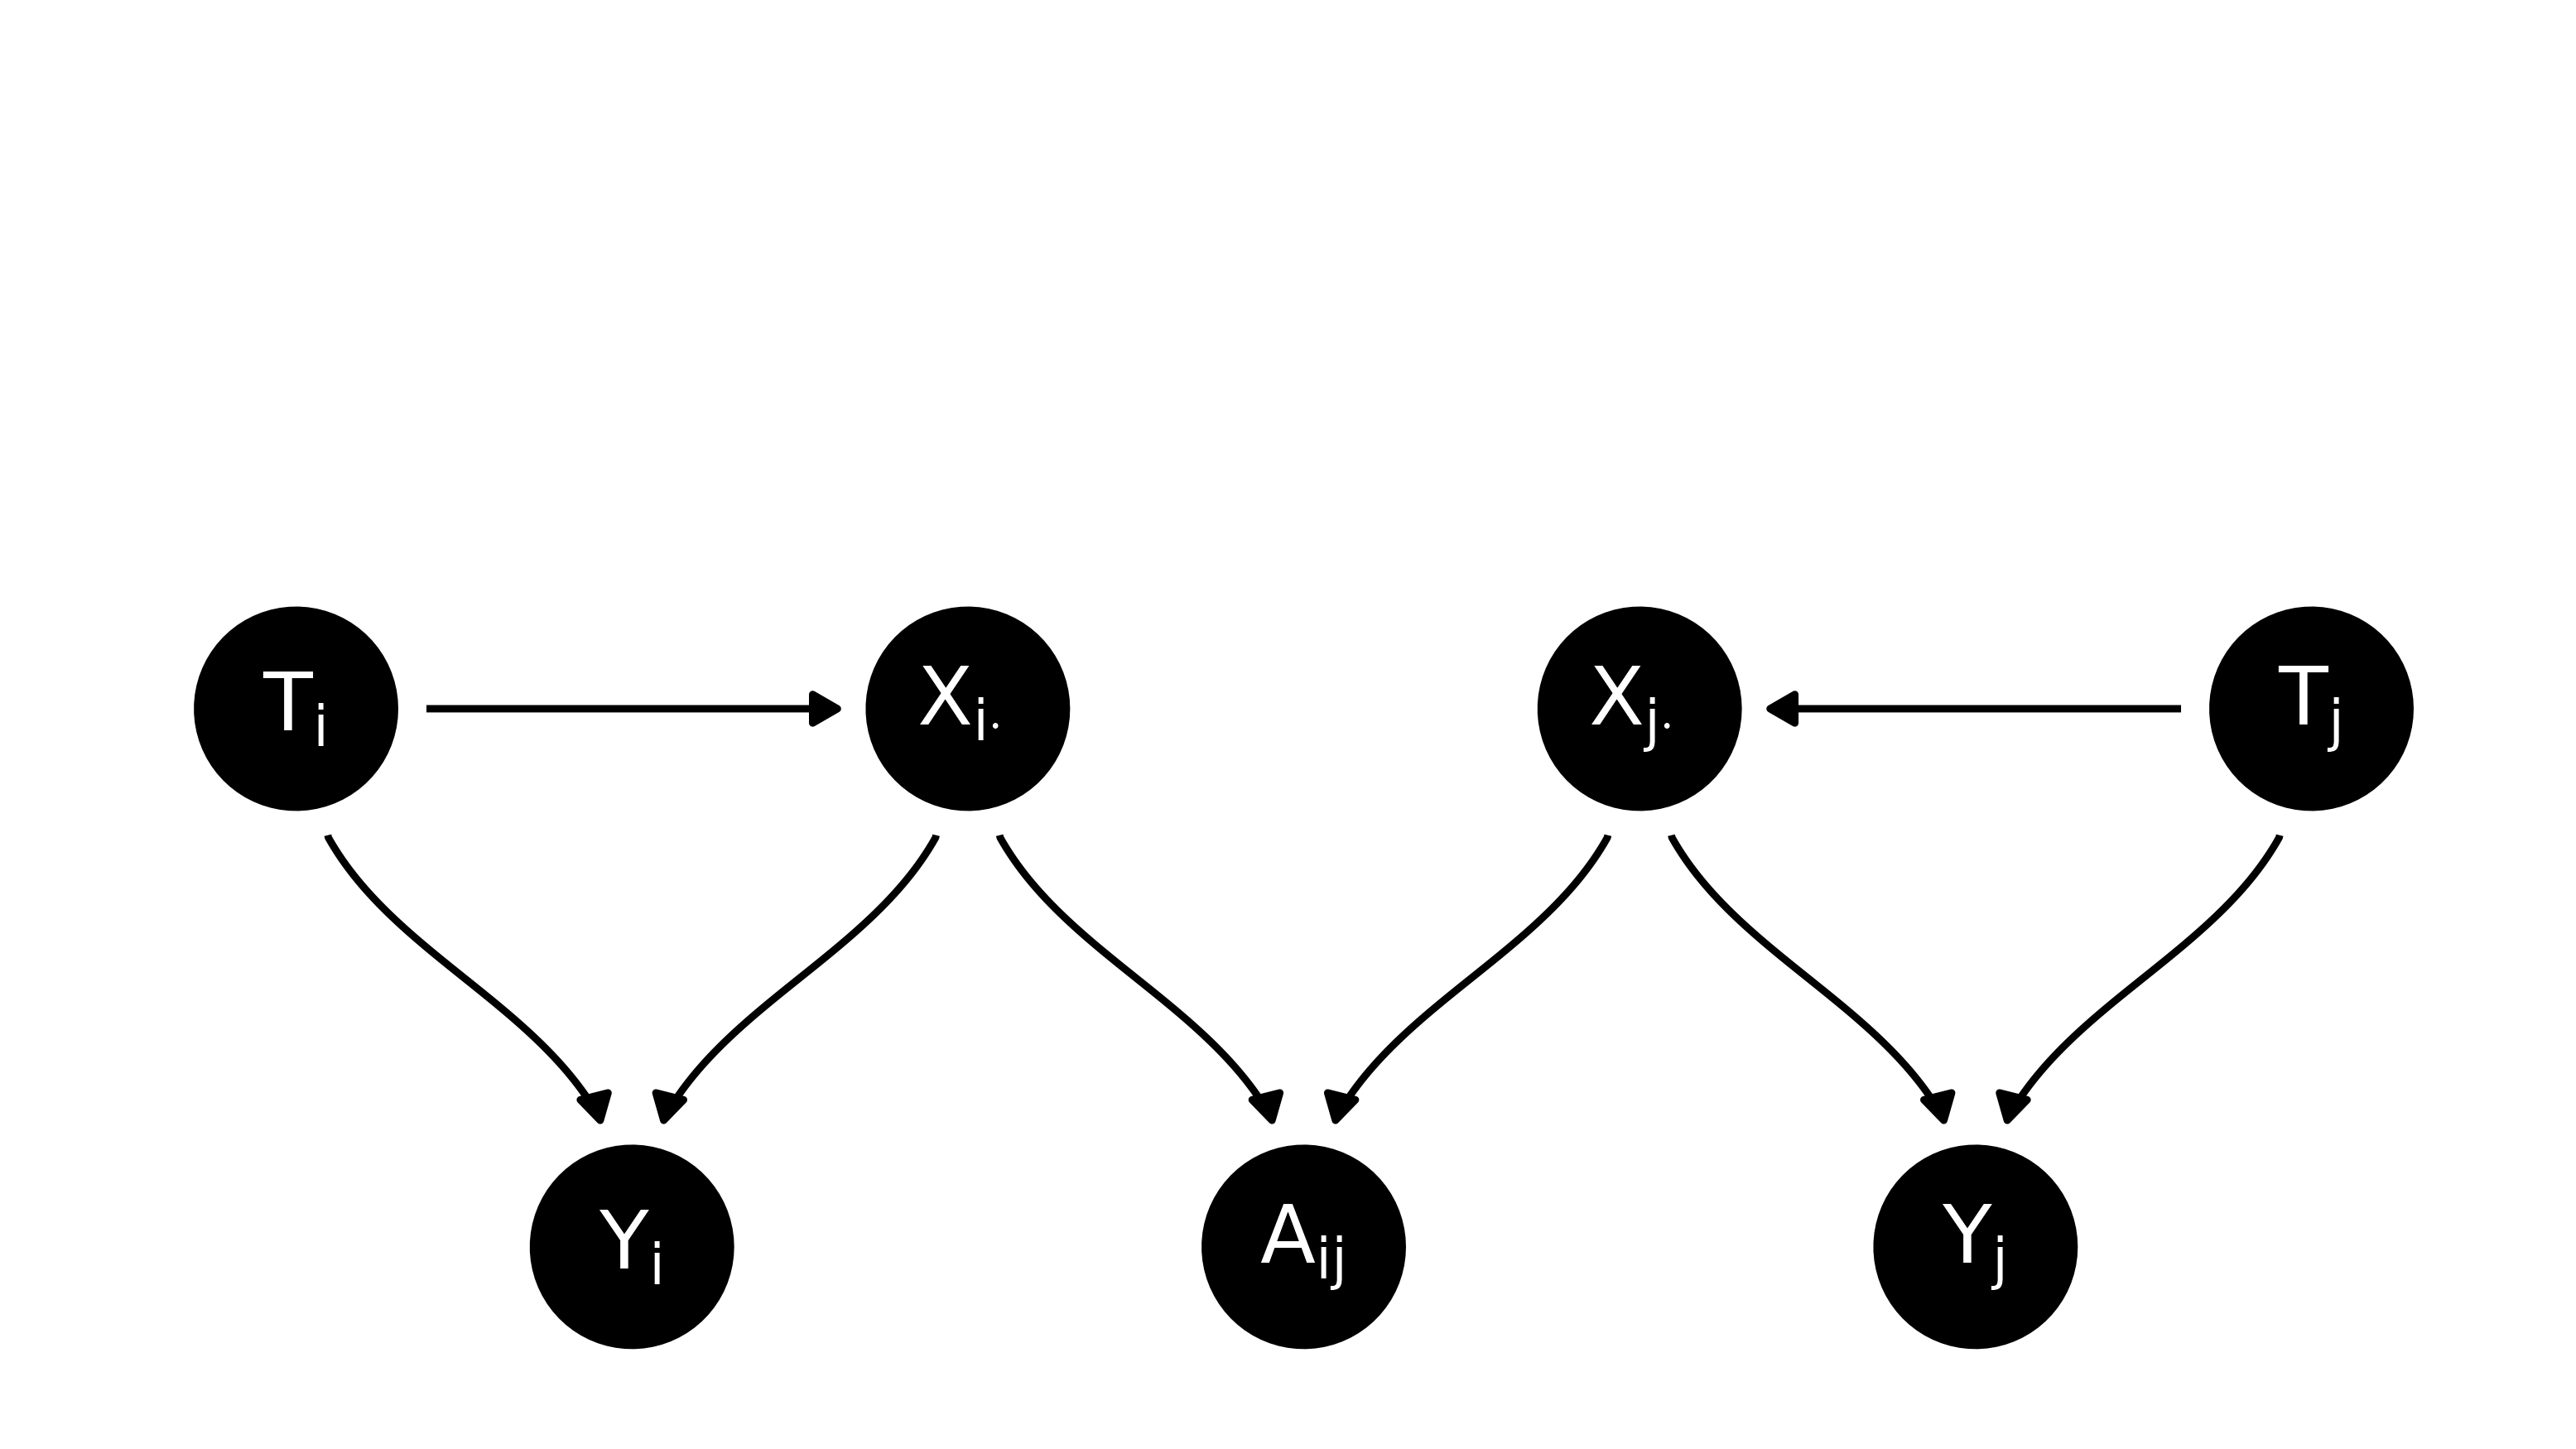
\includegraphics[scale=0.65]{figures/dags/mediating-4.png}
        \label{fig:mediating-4}
    \end{figure}

    i.e. if I want to watch frisbee at the Great Dane

\end{frame}

\begin{frame}{My individual choices might all be confounded}

    \centering

    \begin{figure}
        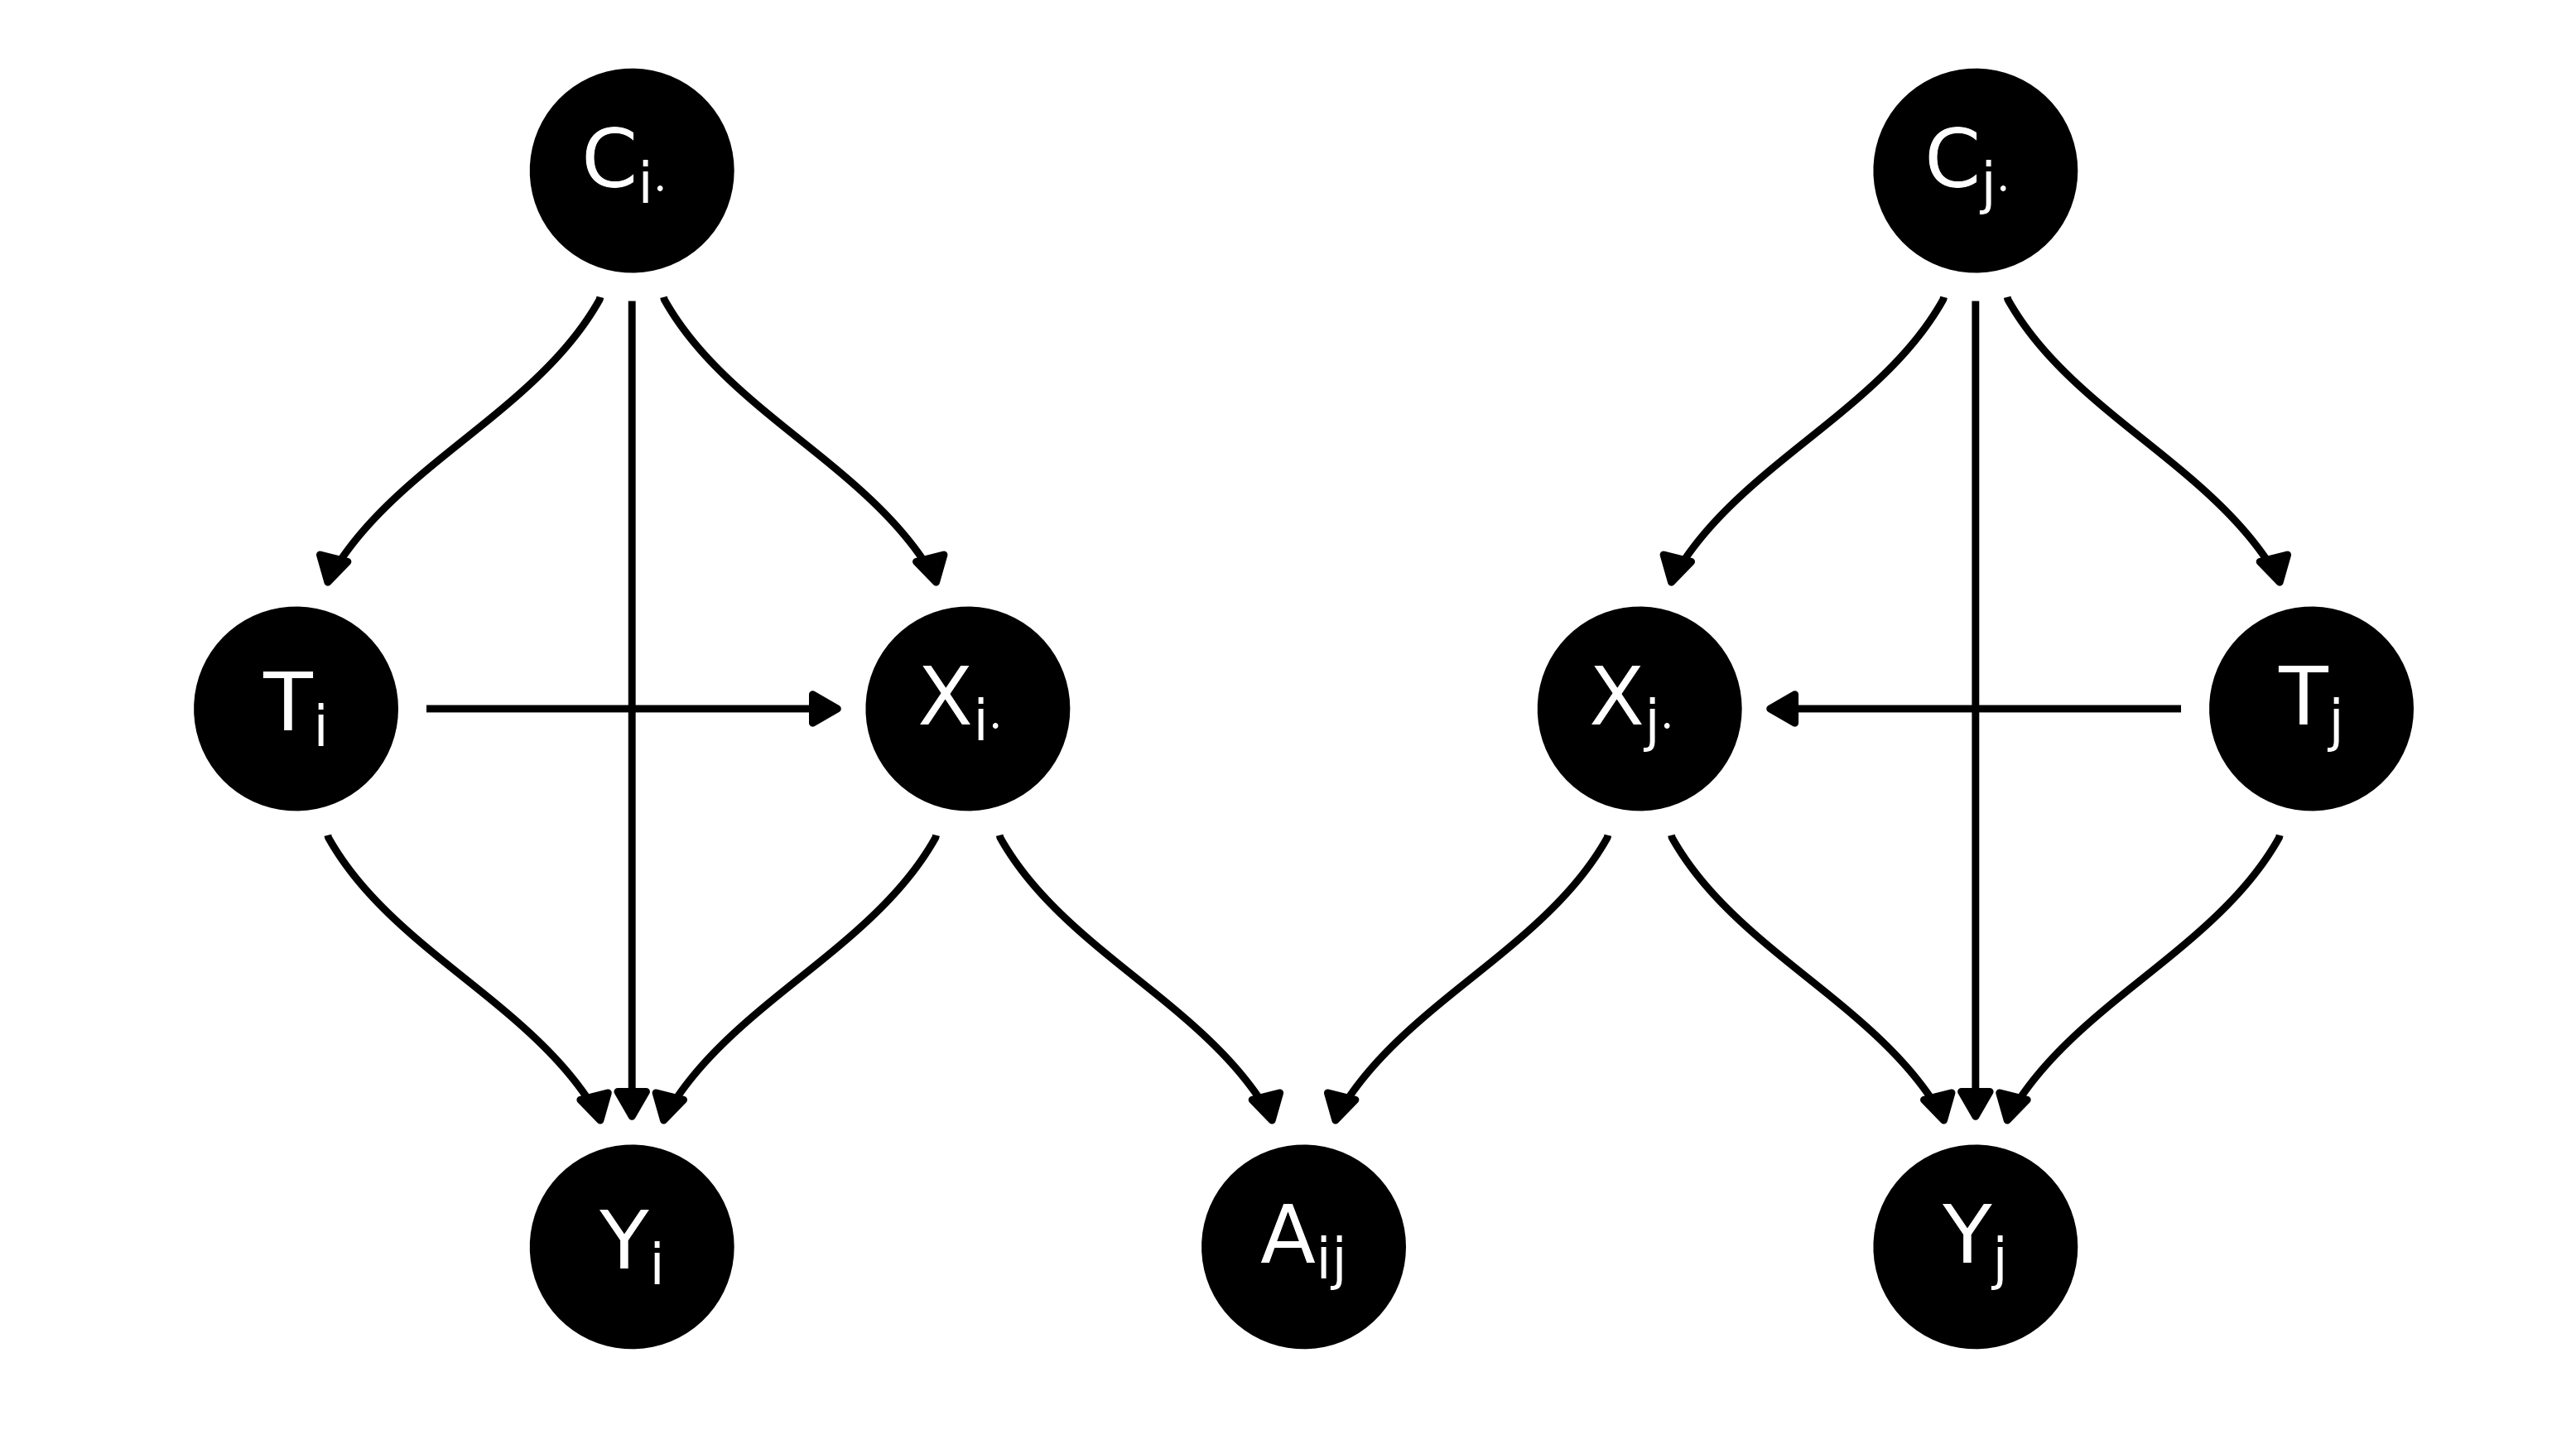
\includegraphics[scale=0.65]{figures/dags/mediating-5.png}
        \label{fig:mediating-5}
    \end{figure}

    This is a good place to ask questions

\end{frame}

\begin{frame}{Formalizing what I think happened with frisbee}

    First, a recap. I think:

    \begin{enumerate}
        \item enjoying frisbee caused me to visit the Great Dane more frequently than I would have otherwise, and

        \item the mechanism proceeded in two stages: first I joined a frisbee team because I liked frisbee, and I went to the Great Dane with the team

        \item I don't think liking frisbee caused me to go to the Great Dane independently of my frisbee team
    \end{enumerate}

    Can disambiguate these causal effects using mediation analysis
\end{frame}

\begin{frame}{Average treatment effect (counterfactual quantity)}

    \begin{itemize}
        \item \emph{Average treatment effect}: how much the outcome $Y$ (Great Dane visits) would change on average if the treatment $T$ were changed from $T = t$ (liking frisbee) to $T = t^*$ (not liking frisbee)
              \begin{equation*}
                  \ate = \E{Y_i(t) - Y_i(t^*)}
              \end{equation*}
    \end{itemize}

    Note: $Y_i(t)$ is the counterfactual value of $Y_i$ when $T_i$ is set to $t$

    I claim $\ate$ is positive in my example

\end{frame}


\begin{frame}{Natural indirect effect (counterfactual quantity)}

    \begin{itemize}
        \item \emph{Natural indirect effect}: how much the outcome $Y$ (Great Dane visits) would change on average if the exposure were fixed at level $T = t^*$ (not liking frisbee) but the mediator $\X$ (friend group) were changed from the level it would take if $T = t$ (liking frisbee) to the level it would take if $T = t^*$ (not liking frisbee)
              \begin{equation*}
                  \nie = \E{Y_i (t, \X_{i \cdot}(t)) - Y_i (t, \X_{i \cdot} (t^*))}
              \end{equation*}
        \item Captures the effect of the exposure on the outcome that operates by changing the mediator
    \end{itemize}

    I claim $\nie$ is positive in my example

\end{frame}

\begin{frame}{Natural direct effect (counterfactual quantity)}

    \begin{itemize}
        \item \emph{Natural direct effect}: how much the outcome $Y$ (Great Dane visits) would change if the exposure $T$ were set at level $T = t^*$ (liking frisbee) versus $T = t$ (liking frisbee) but for each individual the mediator $\X$ (friend group) were kept at the level it would have taken, for that individual, if $T$ had been set to $t^*$ (not liking frisbee)
              \begin{equation*}
                  \nde = \E{Y_i (t, \X_{i \cdot}(t^*)) - Y_i (t^*, \X_{i \cdot} (t^*))}
              \end{equation*}
        \item Captures the effect of the exposure on the outcome that would remain if we were to disable the pathway from the exposure to the mediator
    \end{itemize}

    I claim $\nde$ is zero in my example.

    Note $\ate = \nde + \nie$.

\end{frame}

\begin{frame}{If we knew the friend groups $\X$, we could use standard tools for causal mediation analysis. But we don't know $\X$! Instead, we observe the friendship network $A$}

    \centering

    \begin{figure}
        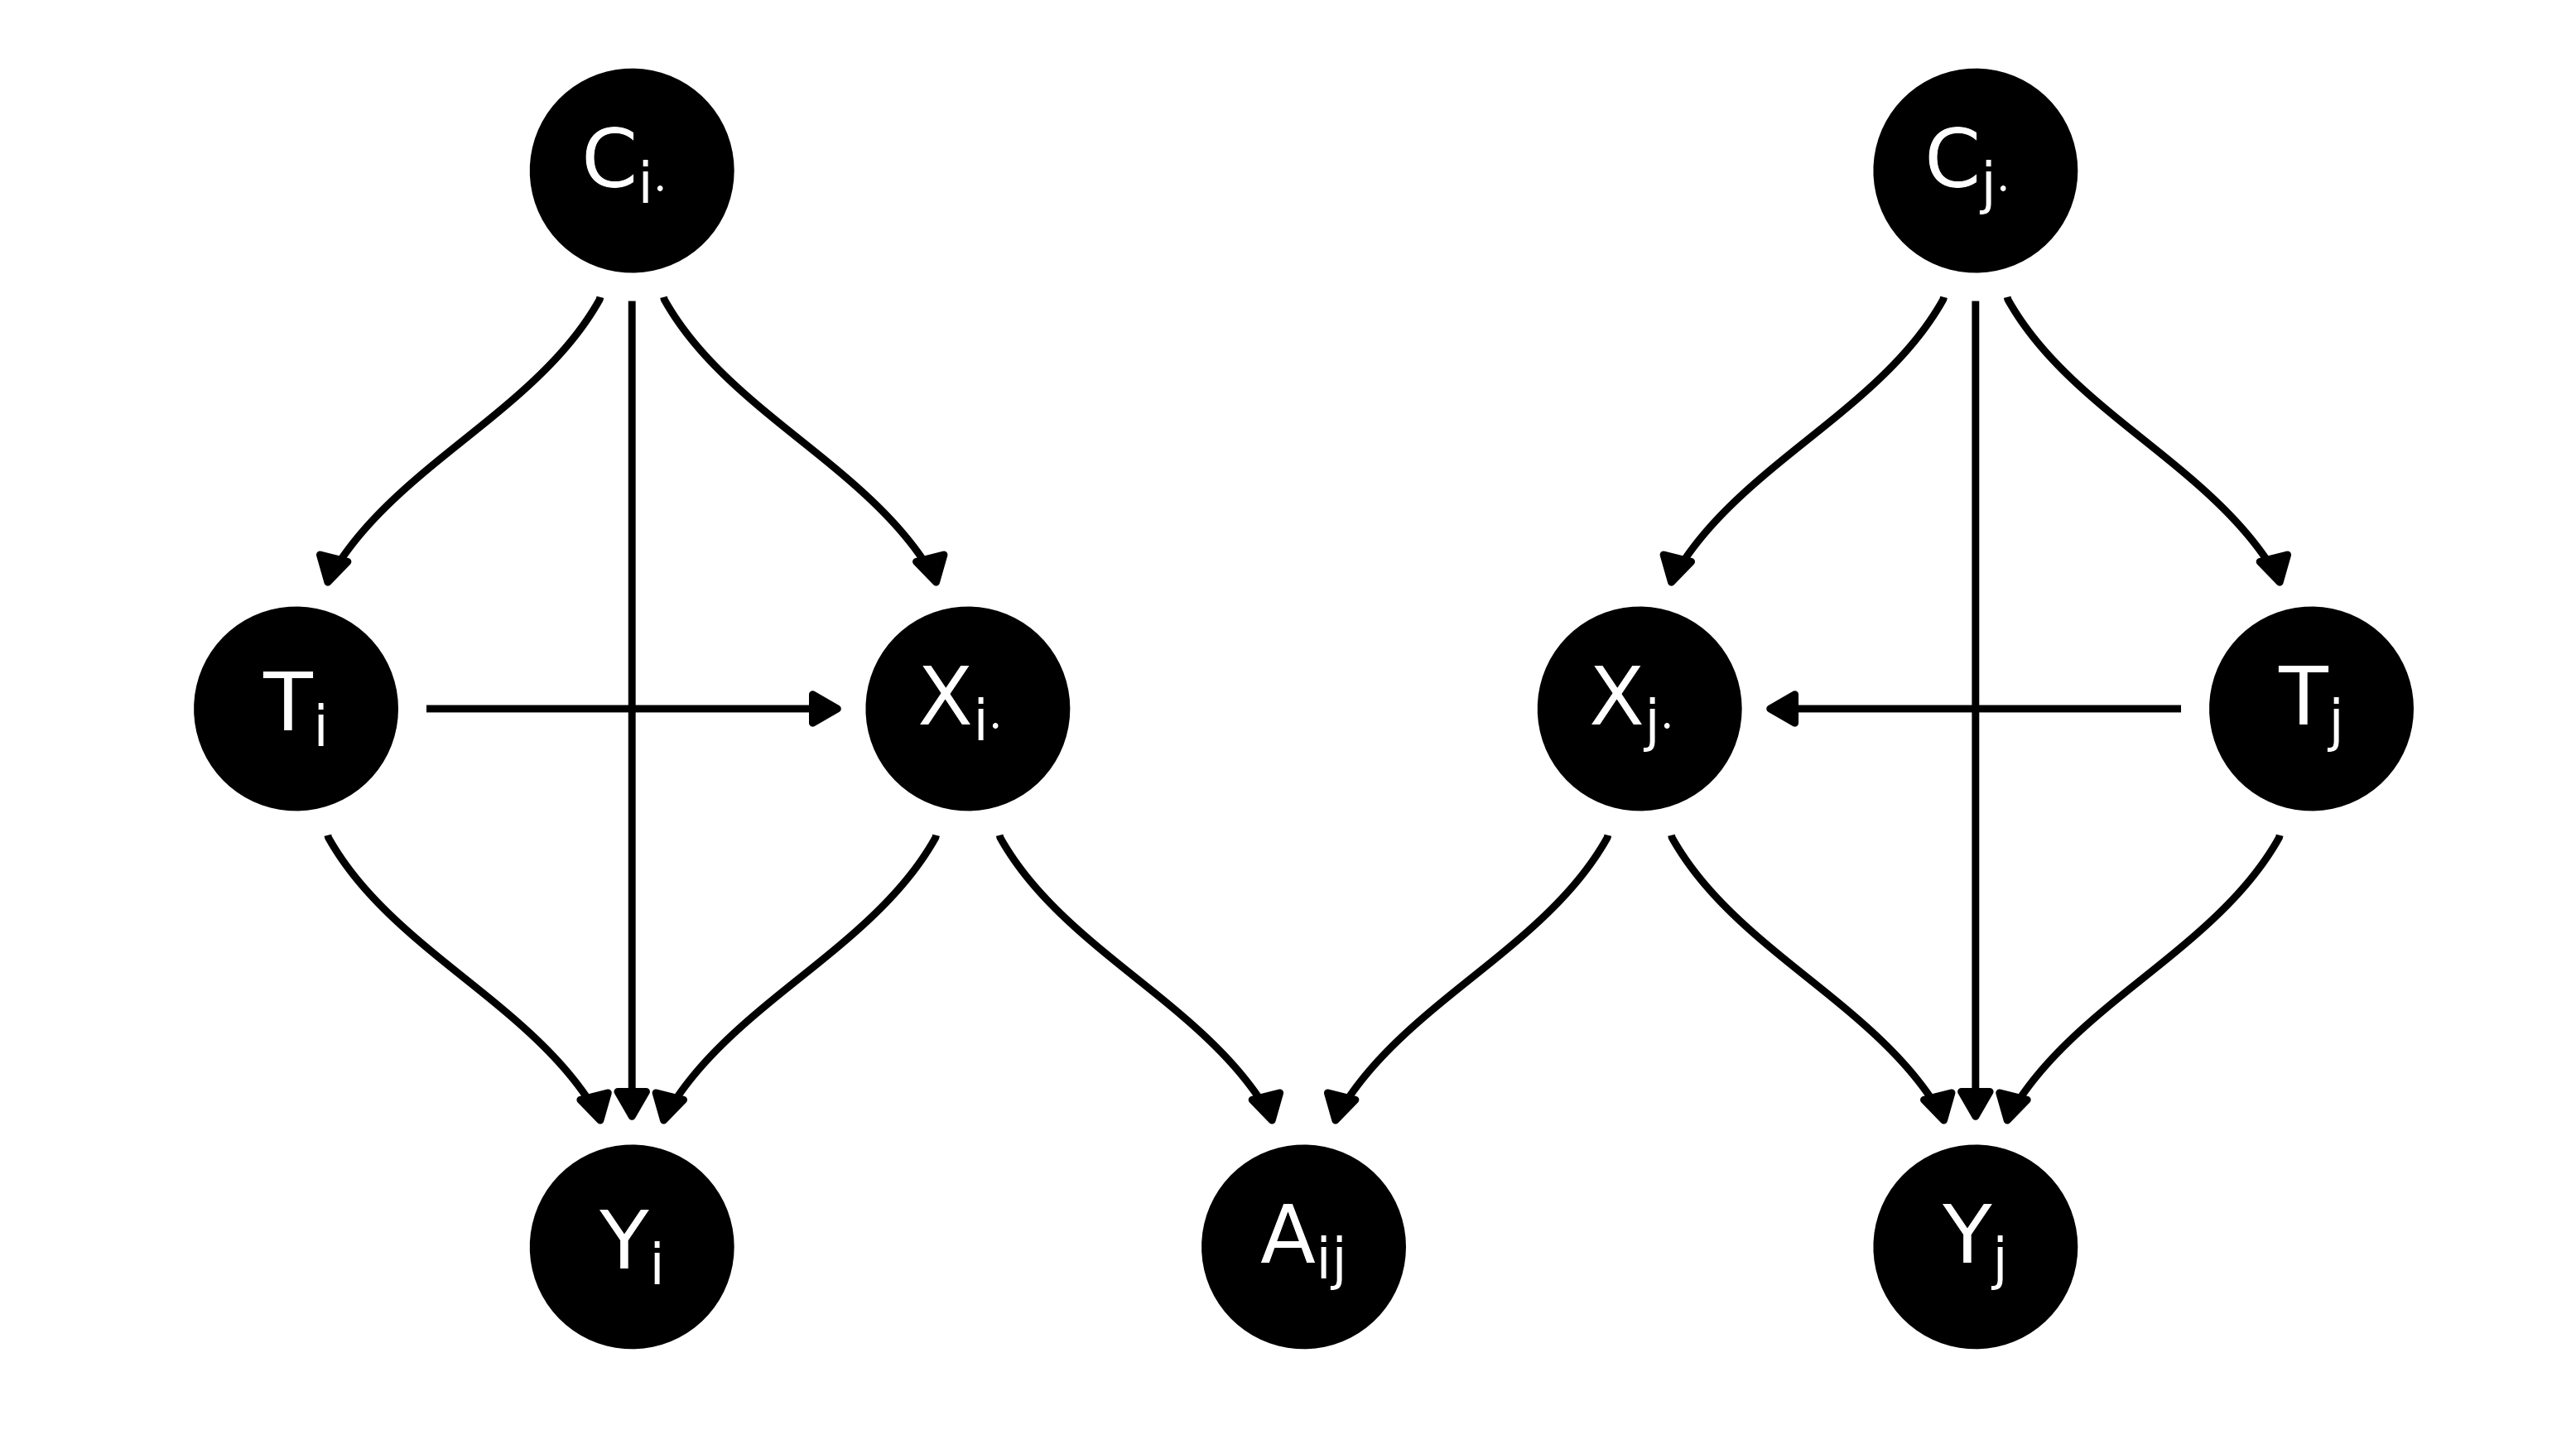
\includegraphics[scale=0.65]{figures/dags/mediating-5.png}
        \label{fig:mediating-5-again}
    \end{figure}

\end{frame}

\section{Semi-parametric network \& network regression models}

\begin{frame}{Intuition: stochastic blockmodels}

    \begin{columns}
        \column{0.45\textwidth}

        \begin{figure}
            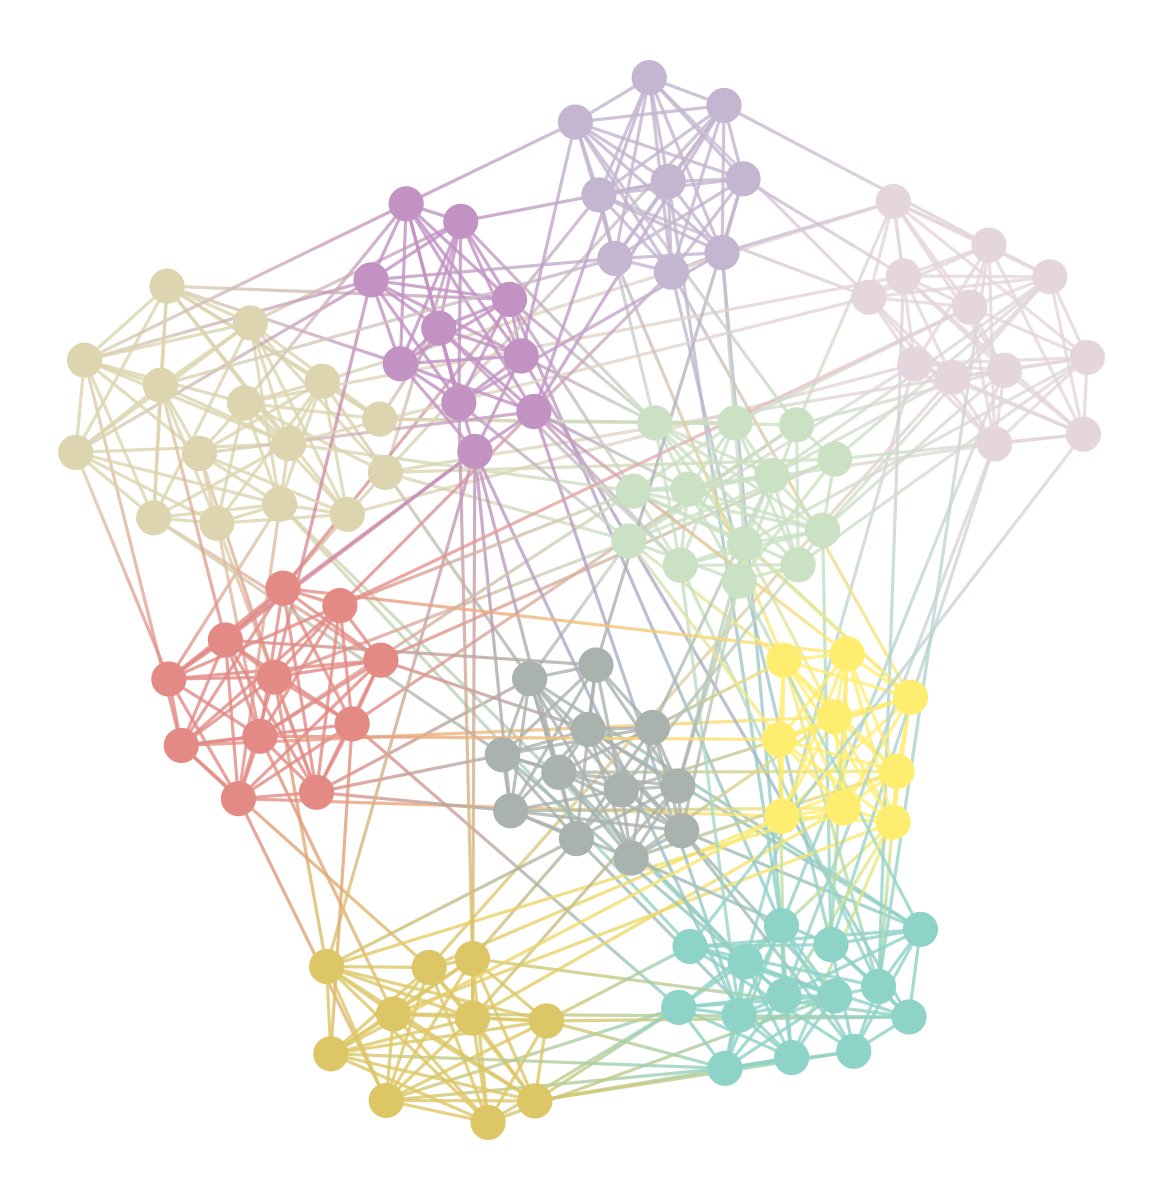
\includegraphics[width=\textwidth]{figures/assortative.png}
        \end{figure}

        \column{0.55\textwidth}

        $d$ ``blocks'' or communities

        $\X_{i \cdot} \in \set{0, 1}^d$ one-hot indicator of node $i$'s block

        \vspace{4mm}

        $\X$ is latent (i.e. unobserved)

        \vspace{4mm}

        $B \in [0, 1]^{d \times d}$ inter-block edge probabilities

        \vspace{4mm}

        Friendships depend on group memberships and $B$

        $\P[\X]{A_{ij} = 1} = \X_{i \cdot} B \X_{j \cdot}^T$

    \end{columns}

\end{frame}

\begin{frame}{Returning to the structural causal model for a moment}

    \centering

    \begin{figure}
        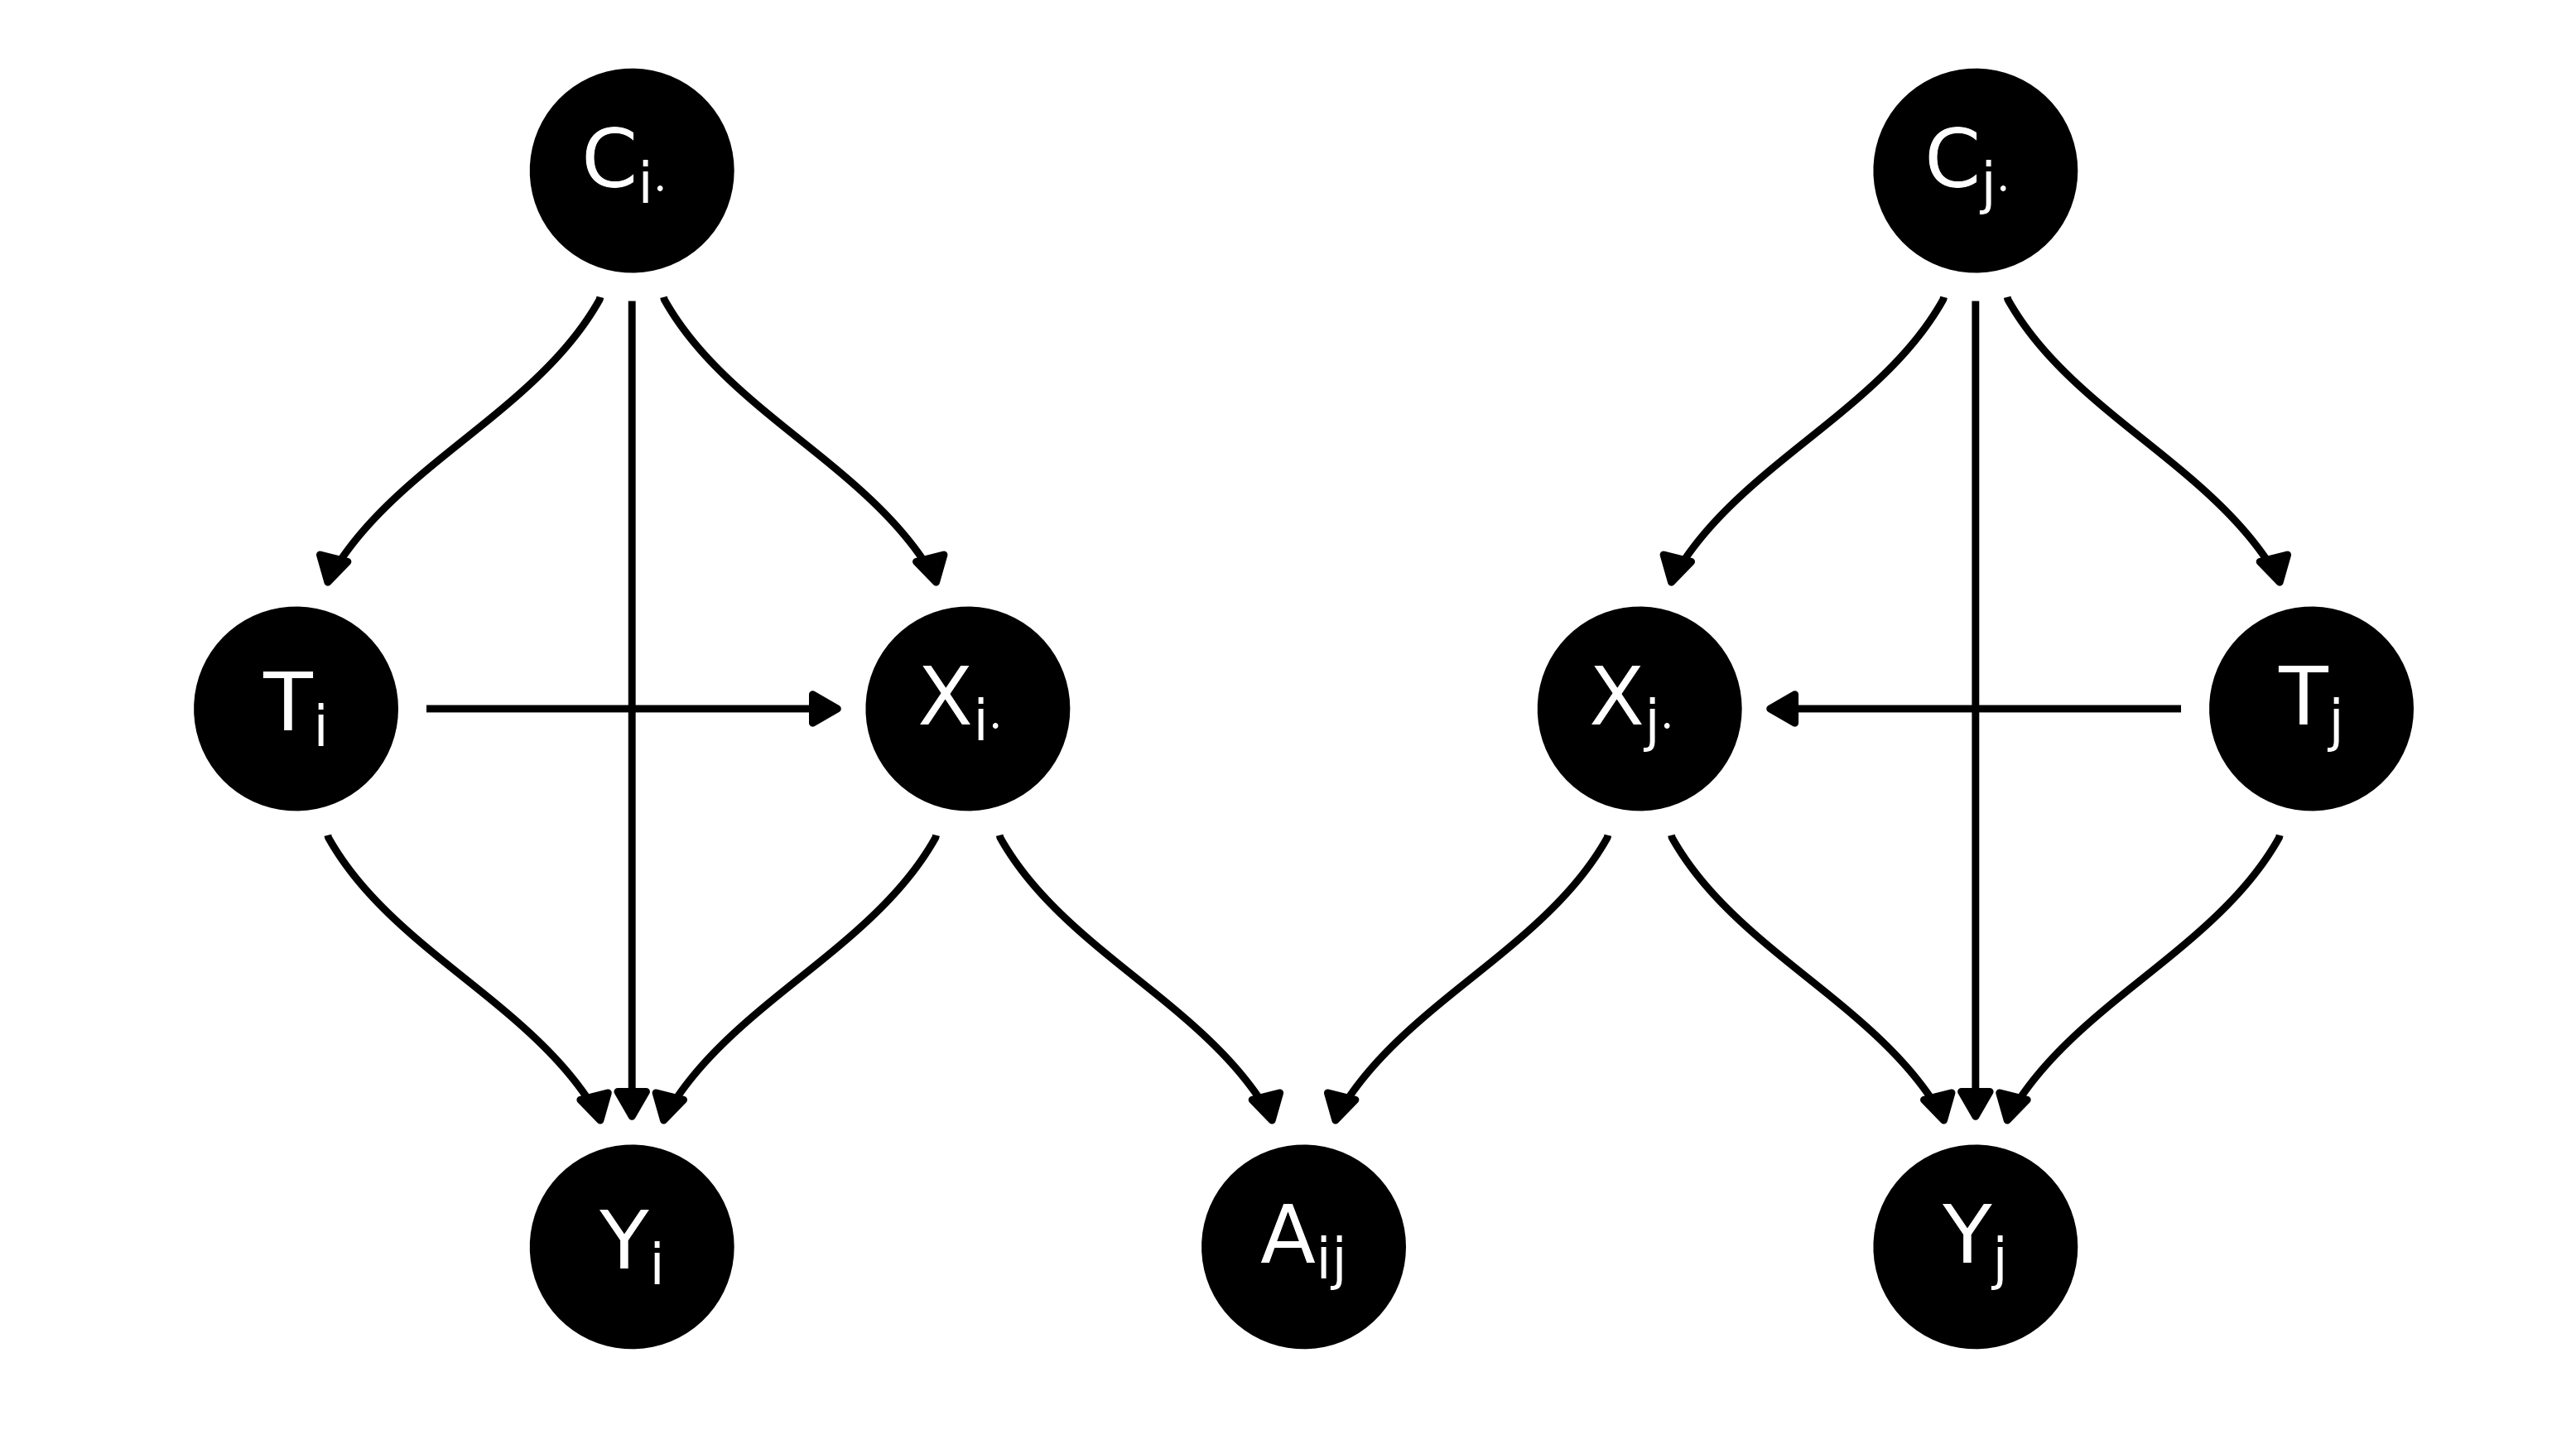
\includegraphics[scale=0.65]{figures/dags/mediating-5.png}
        \label{fig:mediating-5-again}
    \end{figure}

\end{frame}

\begin{frame}{A regression model for friend group membership}

    \centering

    \begin{figure}
        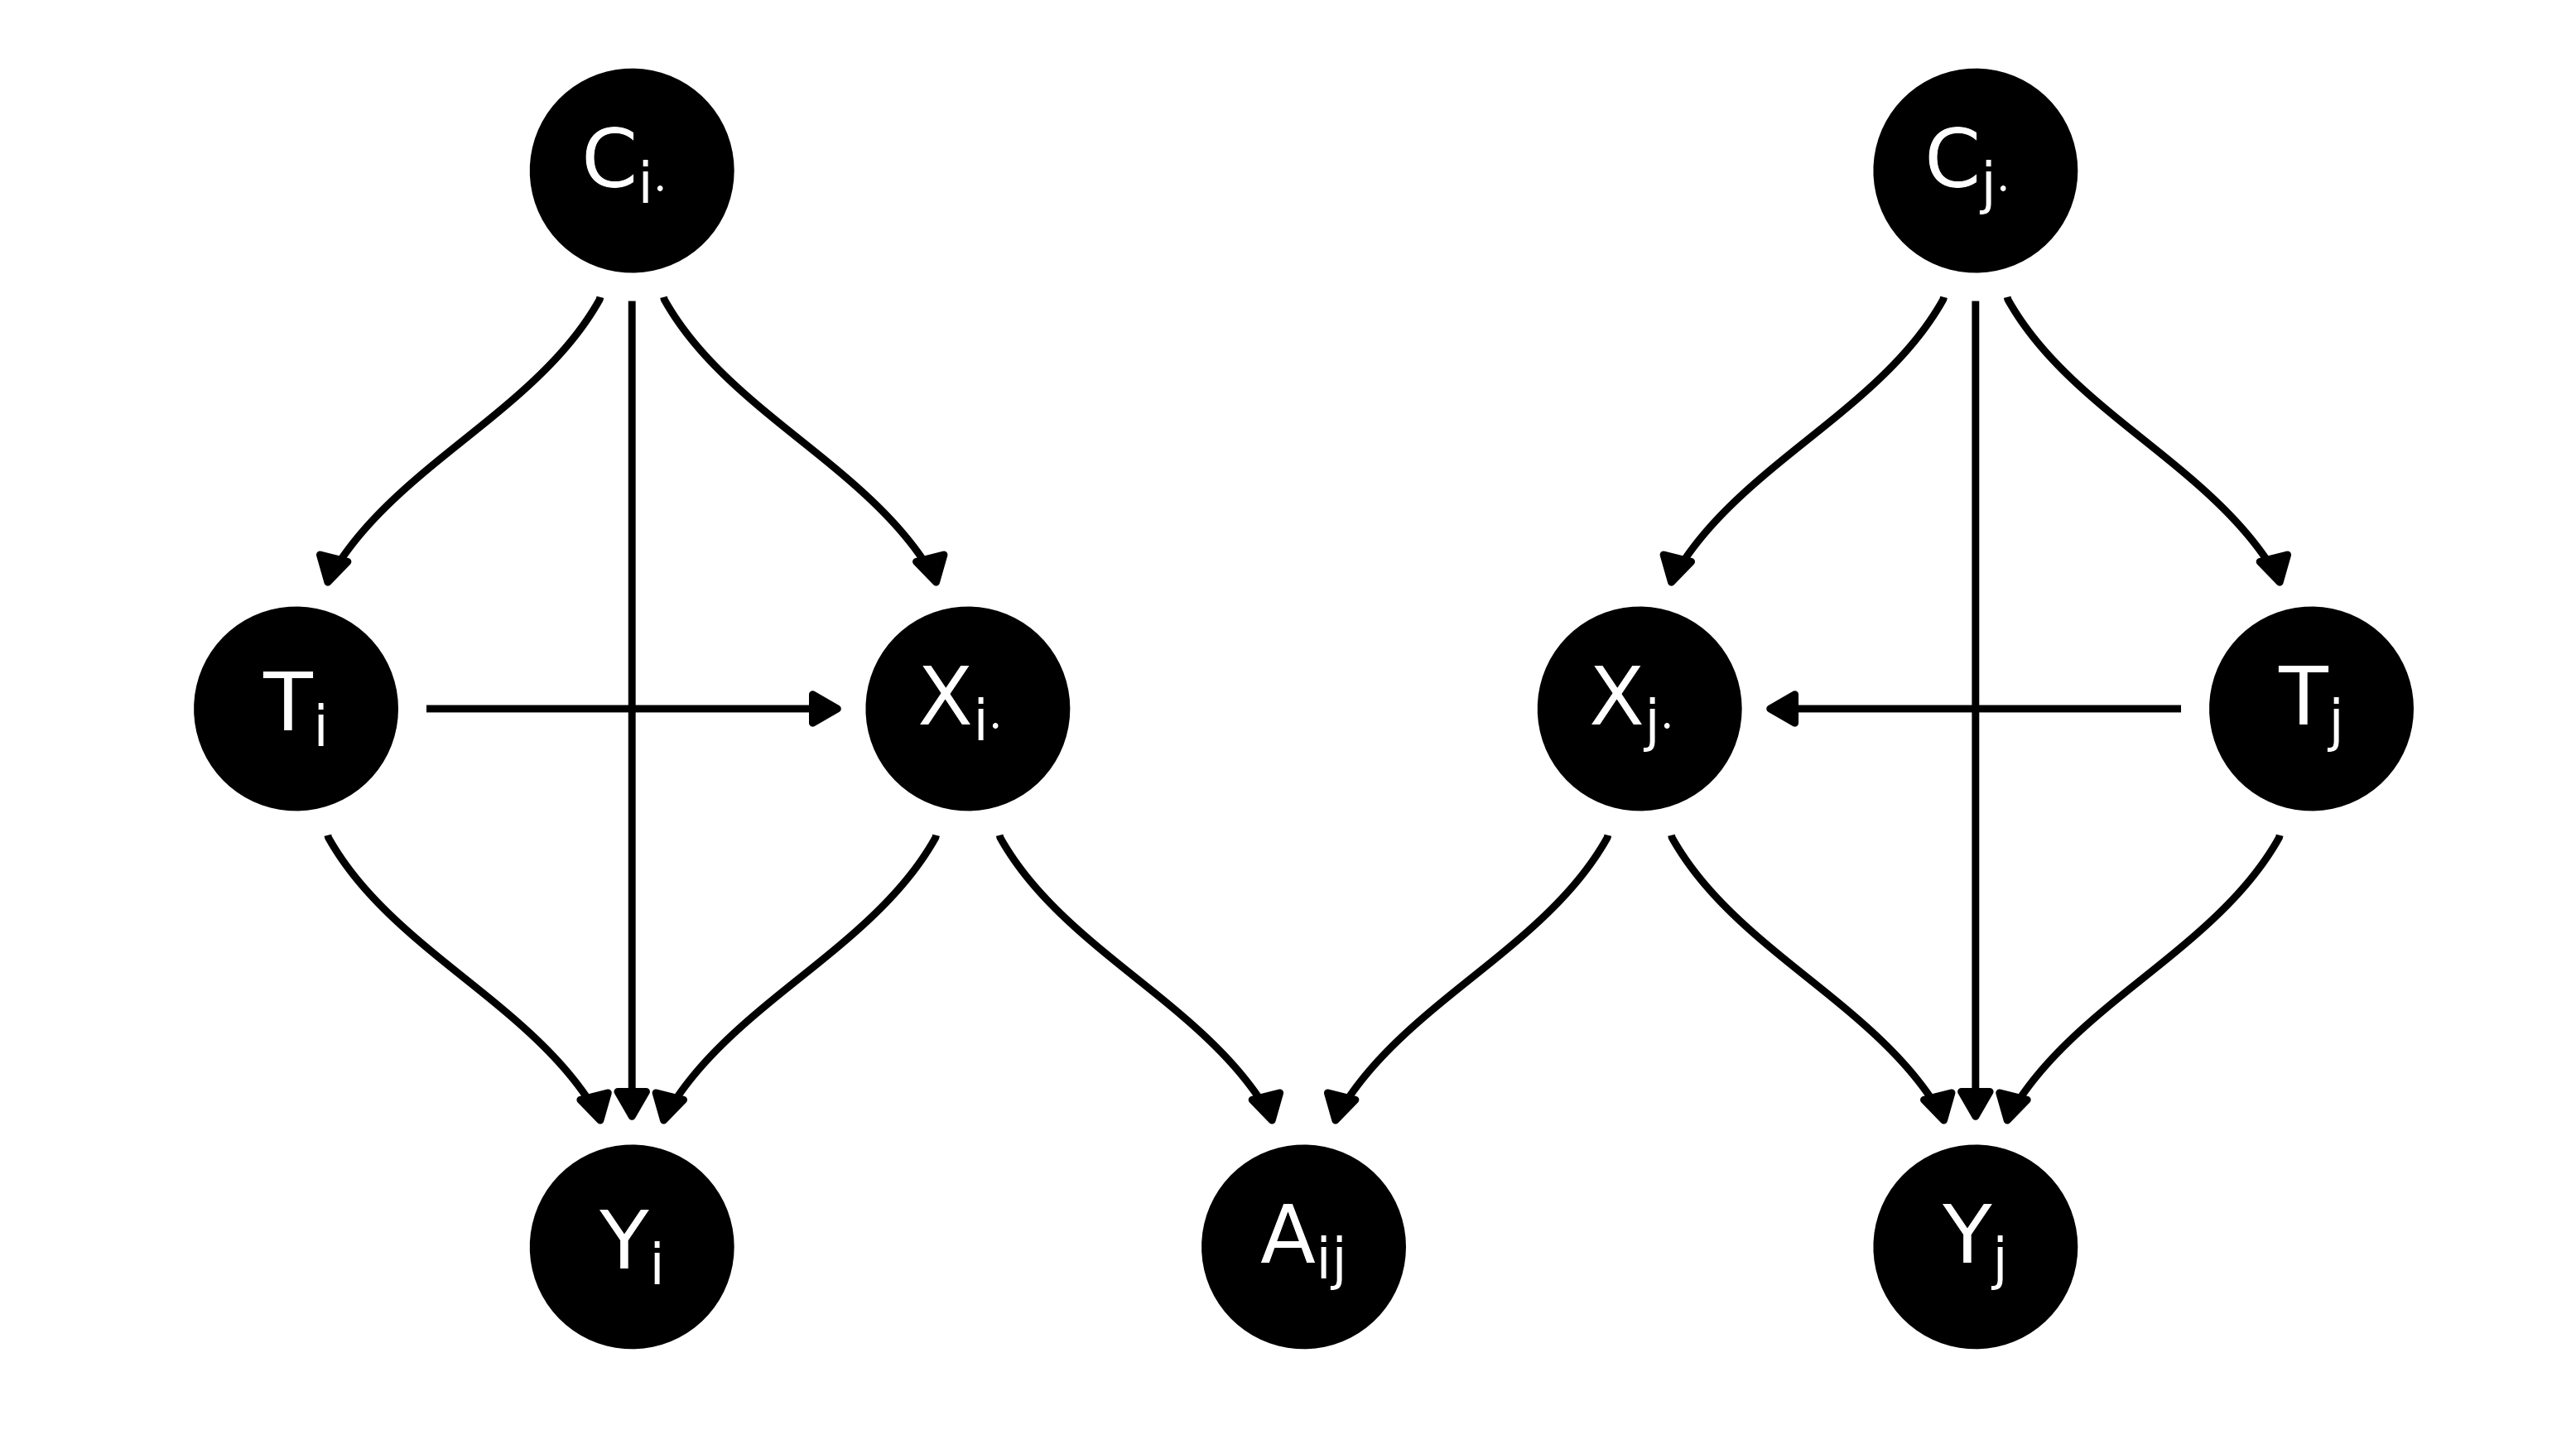
\includegraphics[scale=0.35]{figures/dags/mediating-5.png}
        \label{fig:mediating-5-again}
    \end{figure}
    Idea: interventions $T_i$ can cause community membership $\X_{i \cdot}$
    \begin{align*}
        \underbrace{\E[T_i, \C_{i \cdot}]{\X_{i \cdot}}}_{\R^{1 \times d}}
         & = \underbrace{\thetazero}_{\R^{1 \times d}}
        + \underbrace{T_i}_{\{0, 1\}} \underbrace{\thetat}_{\R^{1 \times d}}
        + \underbrace{\C_{i \cdot}}_{\R^{1 \times p}} \underbrace{\Thetac}_{\R^{p \times d}}
        + \underbrace{T_i}_{\{0, 1\}} \underbrace{\C_{i \cdot}}_{\R^{1 \times p}} \underbrace{\Thetatc}_{\R^{p \times d}}.
    \end{align*}
    Ex: I like frisbee so I joined an ultimate frisbee team (MUFA)

\end{frame}

\begin{frame}{A regression model for outcomes}

    \centering

    \begin{figure}
        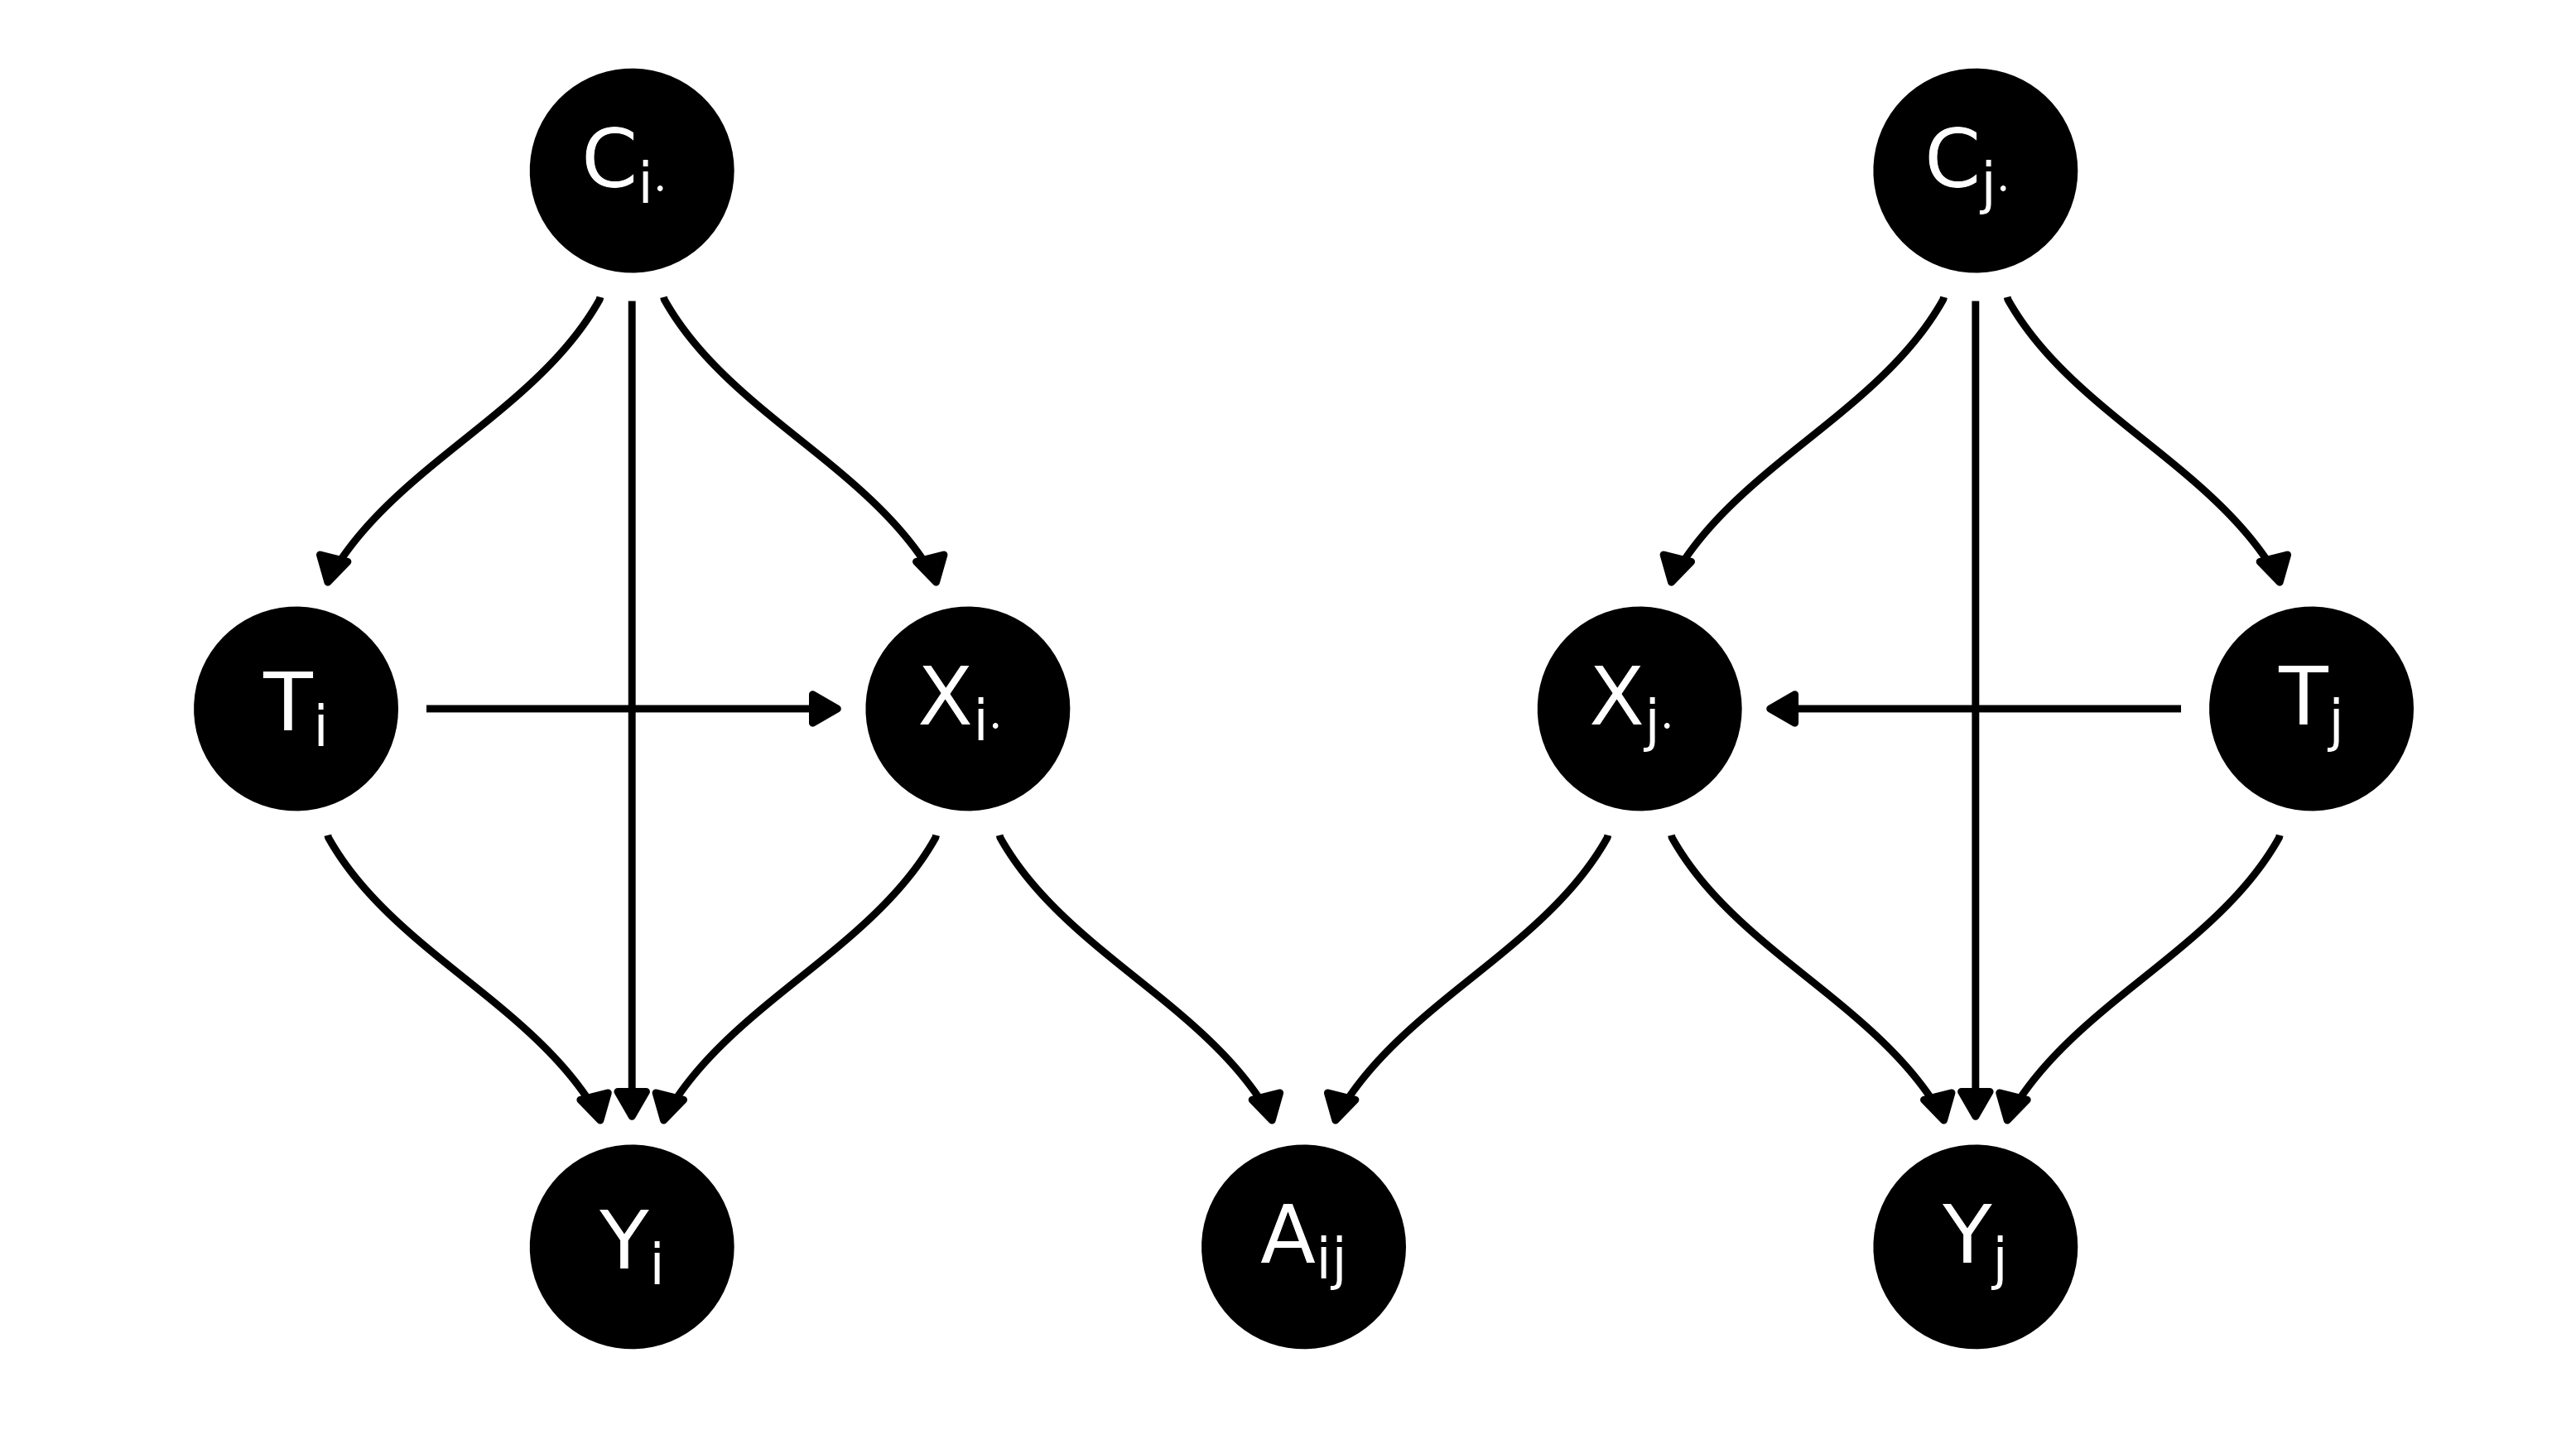
\includegraphics[scale=0.35]{figures/dags/mediating-5.png}
        \label{fig:mediating-5-again}
    \end{figure}

    Idea: community membership $\X_{i \cdot}$ can cause outcomes $Y_i$
    \begin{align*}
        \underbrace{\E[T_i, \C_{i \cdot}, \X_{i \cdot}]{Y_i}}_{\R}
         & = \underbrace{\betazero}_{\R}
        + \underbrace{T_i}_{\{0, 1\}} \underbrace{\betat}_{\R}
        + \underbrace{\C_{i \cdot}}_{\R^{1 \times p}} \underbrace{\betac}_{\R^{p}}
        + \underbrace{\X_{i \cdot}}_{\R^{1 \times d}} \underbrace{\betax}_{\R^d}
    \end{align*}
    Ex: I'm on a frisbee team, and the frisbee team goes to the Great Dane together after each game

\end{frame}

\begin{frame}{Semi-parametric causal identification}

    Recall the regression models:
    \begin{equation*}
        \begin{aligned}
            \underbrace{\E[T_i, \C_{i \cdot}, \X_{i \cdot}]{Y_i}}_{\R}
             & = \underbrace{\betazero}_{\R}
            + \underbrace{T_i}_{\{0, 1\}} \underbrace{\betat}_{\R}
            + \underbrace{\C_{i \cdot}}_{\R^{1 \times p}} \underbrace{\betac}_{\R^{p}}
            + \underbrace{\X_{i \cdot}}_{\R^{1 \times d}} \underbrace{\betax}_{\R^d}, \\
            \underbrace{\E[T_i, \C_{i \cdot}]{\X_{i \cdot}}}_{\R^{1 \times d}}
             & = \underbrace{\thetazero}_{\R^{1 \times d}}
            + \underbrace{T_i}_{\{0, 1\}} \underbrace{\thetat}_{\R^{1 \times d}}
            + \underbrace{\C_{i \cdot}}_{\R^{1 \times p}} \underbrace{\Thetac}_{\R^{p \times d}}
            + \underbrace{T_i}_{\{0, 1\}} \underbrace{\C_{i \cdot}}_{\R^{1 \times p}} \underbrace{\Thetatc}_{\R^{p \times d}}.
        \end{aligned}
    \end{equation*}
    Then:
    \begin{align*}
        \ndef & = \paren*{t - t^*} \, \betat                                                        \\
        \nief & = \paren*{t - t^*} \, \thetat \, \betax + (t - t^*) \, \mu_c \, \Thetatc \, \betax.
    \end{align*}

\end{frame}

\section{Estimation}

\begin{frame}{Regression estimators}

    \textbf{Challenge}: regression models depend on $\X$, but we never see $\X$. Luckily we can estimate it!

    \begin{definition}[ASE]

        Given a network $A$, the $\widehat{d}$-dimensional \emph{adjacency spectral embedding} of $A$ is

        \begin{align*}
            \Xhat = \Uhat \Shat^{1/2}
        \end{align*}

        \noindent where $\Uhat \Shat \Uhat^T$ is the rank-$\widehat{d}$ truncated singular value decomposition of $A$.

    \end{definition}

    \textbf{Note that the analyst must specify $\widehat{d}$}

\end{frame}

\begin{frame}{Uniform consistency of the adjacency spectral embedding}

    Well-known that $\Xhat$ is a good estimate of $\X$

    \begin{lemma}

        Under a suitably well-behaved network model, if $\widehat{d}$ is correctly specified or consistently estimated, there is some $d \times d$ orthogonal matrix $Q$ such that
        \begin{equation*}
            \max_{i \in [n]} \, \norm*{\Xhat_{i \cdot} - \X_{i \cdot} Q} = \op{1}.
        \end{equation*}

    \end{lemma}

\end{frame}


\begin{frame}{$\Xhat$ can be plugged in for $\X$ just fine}

    Let $\Dhat = \begin{bmatrix} 1 & T & \C  & \Xhat \end{bmatrix} \in \R^{n \times (2 + p + d)}$ and $\Wfull = \begin{bmatrix} 1 & T & \C  & T \cdot \C \end{bmatrix} \in \R^{n \times (2 p + 2)}$.

    We estimate $\betaw$ and $\betax$ via ordinary least squares as follows
    \begin{equation*}
        \begin{bmatrix}
            \betazerohat \\
            \betathat    \\
            \betachat    \\
            \betaxhat
        \end{bmatrix}
        = \paren*{\Dhat^T \Dhat}^{-1} \Dhat^T Y.
    \end{equation*}
    Similarly, we estimate $\Theta$ via ordinary least squares as
    \begin{equation*}
        \Thetahat
        = \paren*{\Wfull^T \Wfull}^{-1} \Wfull^T \Xhat.
    \end{equation*}
\end{frame}

\begin{frame}{Causal estimators}

    To estimate $\nde$ and $\nie$ in our semi-parametric setting, we combine regression coefficients from the network regression models:
    \begin{align*}
        \cdehat & = \ndehat = \paren*{t - t^*} \, \betathat                                                                              & \text{and} \\
        \niehat & = \paren*{t - t^*} \, \thetathat \, \betaxhat + \paren*{t - t^*} \cdot \widehat{\mu}_c \cdot \Thetatchat \, \betaxhat.
    \end{align*}
    It's standard to fit two regressions and multiply coefficients to estimate an indirect effect like this \citep{vanderweele_mediation_2014}.

\end{frame}

\begin{frame}{Main result}

    \begin{theorem}[Regression coefficients are asymptotically normal]

        \vspace{2mm}

        Under some mild assumptions, there is some unknown matrix $Q$ such that
        \begin{equation*}
            \begin{aligned}
                \sqrt{ n } \,
                 & \Sigmahatbeta^{-1/2}
                \begin{pmatrix}
                    \betawhat - \betaw \\
                    Q \, \betaxhat - \betax
                \end{pmatrix}
                \to
                \Normal{0}{I_d}, and     \\
                \sqrt{ n } \,
                 & \Sigmahattheta^{-1/2}
                \begin{pmatrix}
                    \vecc \paren*{\Thetahat \, Q^T} - \Thetavec
                \end{pmatrix}
                \to
                \Normal{0}{I_{p d}}.
            \end{aligned}
        \end{equation*}
        \noindent where $\Sigmahattheta^{-1/2}$ and $\Sigmahatbeta^{-1/2}$ are the typical heteroscedasticity robust covariance estimators, with $\Xhat$ plugged in for $\X$.
    \end{theorem}
\end{frame}

\begin{frame}{Corollary}

    \begin{theorem}[Causal estimators are asymptotically normal]

        \vspace{2mm}

        Under the same statistical assumptions as before, plus mediating homophily,
        \begin{align*}
            \sqrt{n \, \sigmahatnde} \paren*{\ndehat - \nde}
             & \to
            \Normal{0}{1}, \text { and } \\
            \sqrt{n \, \sigmahatnie} \paren*{\niehat - \nie}
             & \to
            \Normal{0}{1}.
        \end{align*}
        \noindent where $\sigmahatnde$ and $\sigmahatnie$ are rather unfriendly variance estimators derived via the delta method and the previous theorem.

    \end{theorem}

\end{frame}

% \section{Data example (if there is time)}

% \begin{frame}{Glasgow data}

%     TODO

% \end{frame}


\begin{frame}{Thank you! Questions?}

    Read the manuscript at \url{https://arxiv.org/abs/2212.12041}

    Slides available at \url{https://tinyurl.com/ifds-alex}

    R package \href{https://github.com/alexpghayes/netmediate}{netmediate}

    \textbf{Stay in touch}

    \begin{itemize}
        \item[] \faIcon{twitter} \href{https://twitter.com/alexpghayes}{@alexpghayes}
        \item[] \faIcon[regular]{envelope} \href{mailto:alex.hayes@wisc.edu}{alex.hayes@wisc.edu}
        \item[] \faIcon{wordpress} \url{https://www.alexpghayes.com} % \faIcon{sitemap} \faIcon{firefox-browser} 
        \item[] \faIcon{github} \url{https://github.com/alexpghayes}
    \end{itemize}

    \textbf{I'll be on the post-doc market in Fall 2023}
\end{frame}

\appendix

\begin{frame}{Disambiguation: contagion is not allowed}

    \centering

    \begin{figure}
        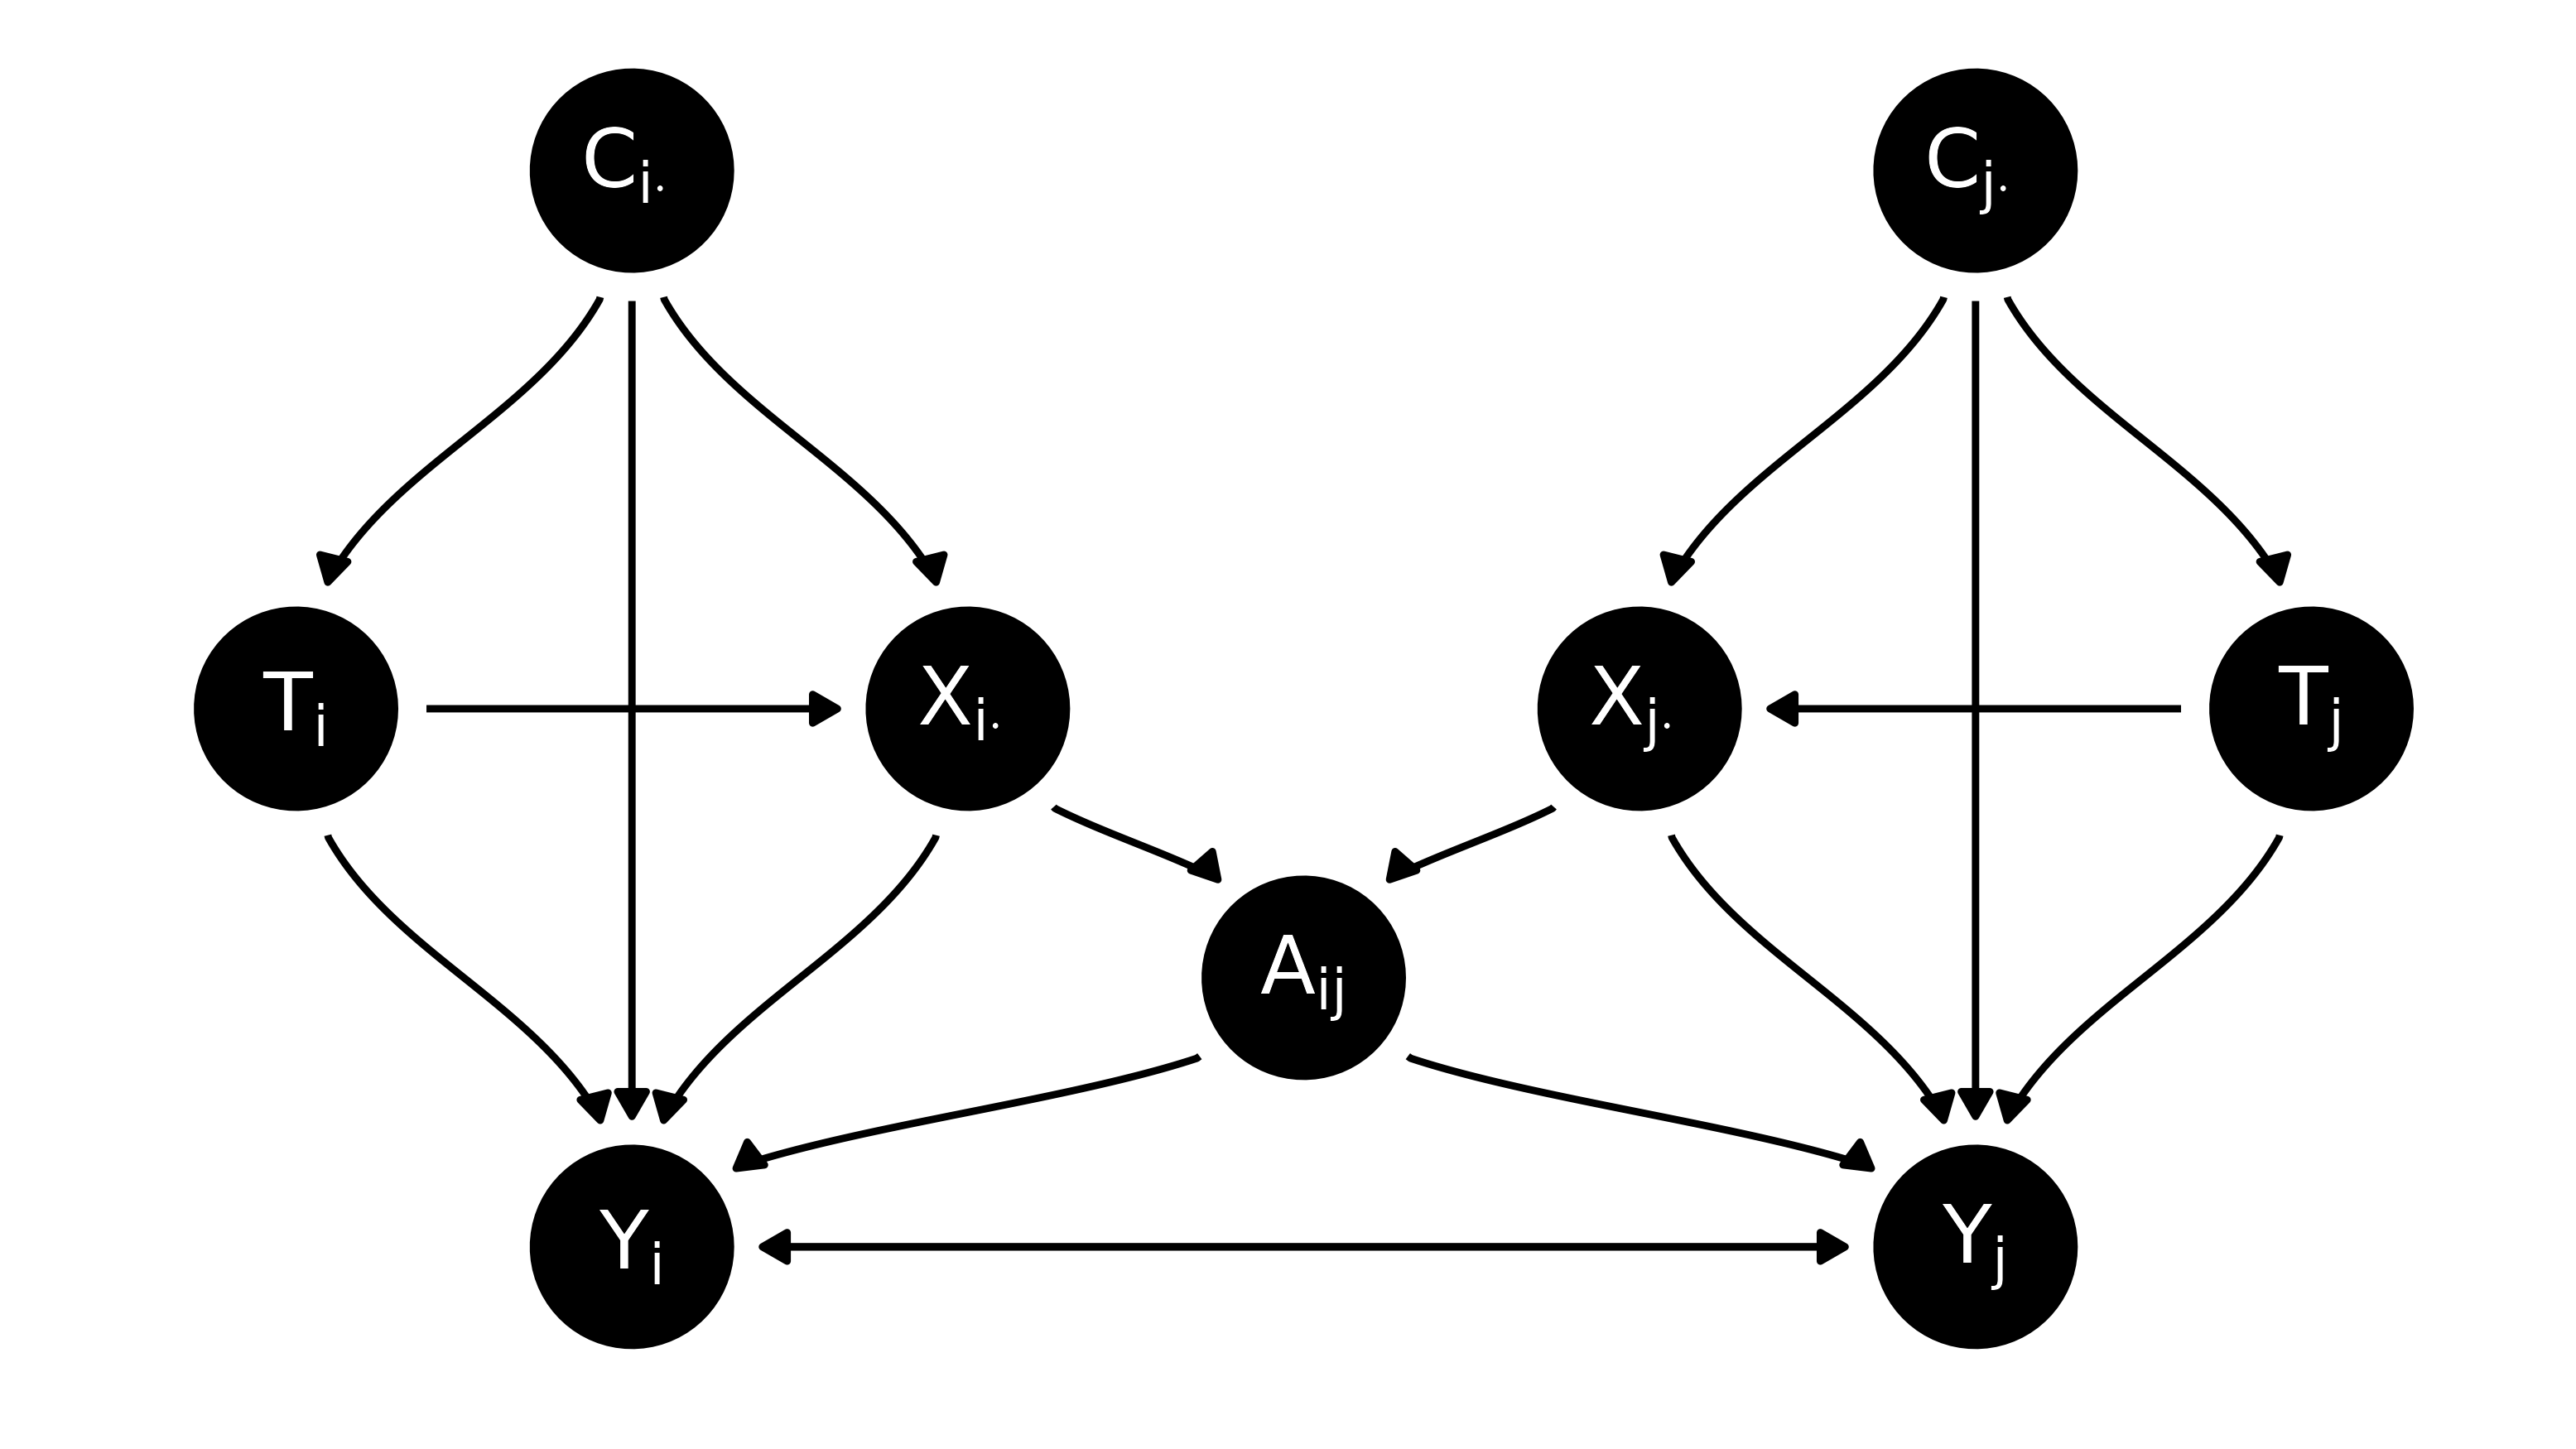
\includegraphics[scale=0.65]{figures/dags/contagion.png}
        \label{fig:contagion}
    \end{figure}

    Contagion ($Y_j \to Y_i$) is not allowed

\end{frame}

\begin{frame}{Disambiguation: interference is not allowed}

    \centering

    \begin{figure}
        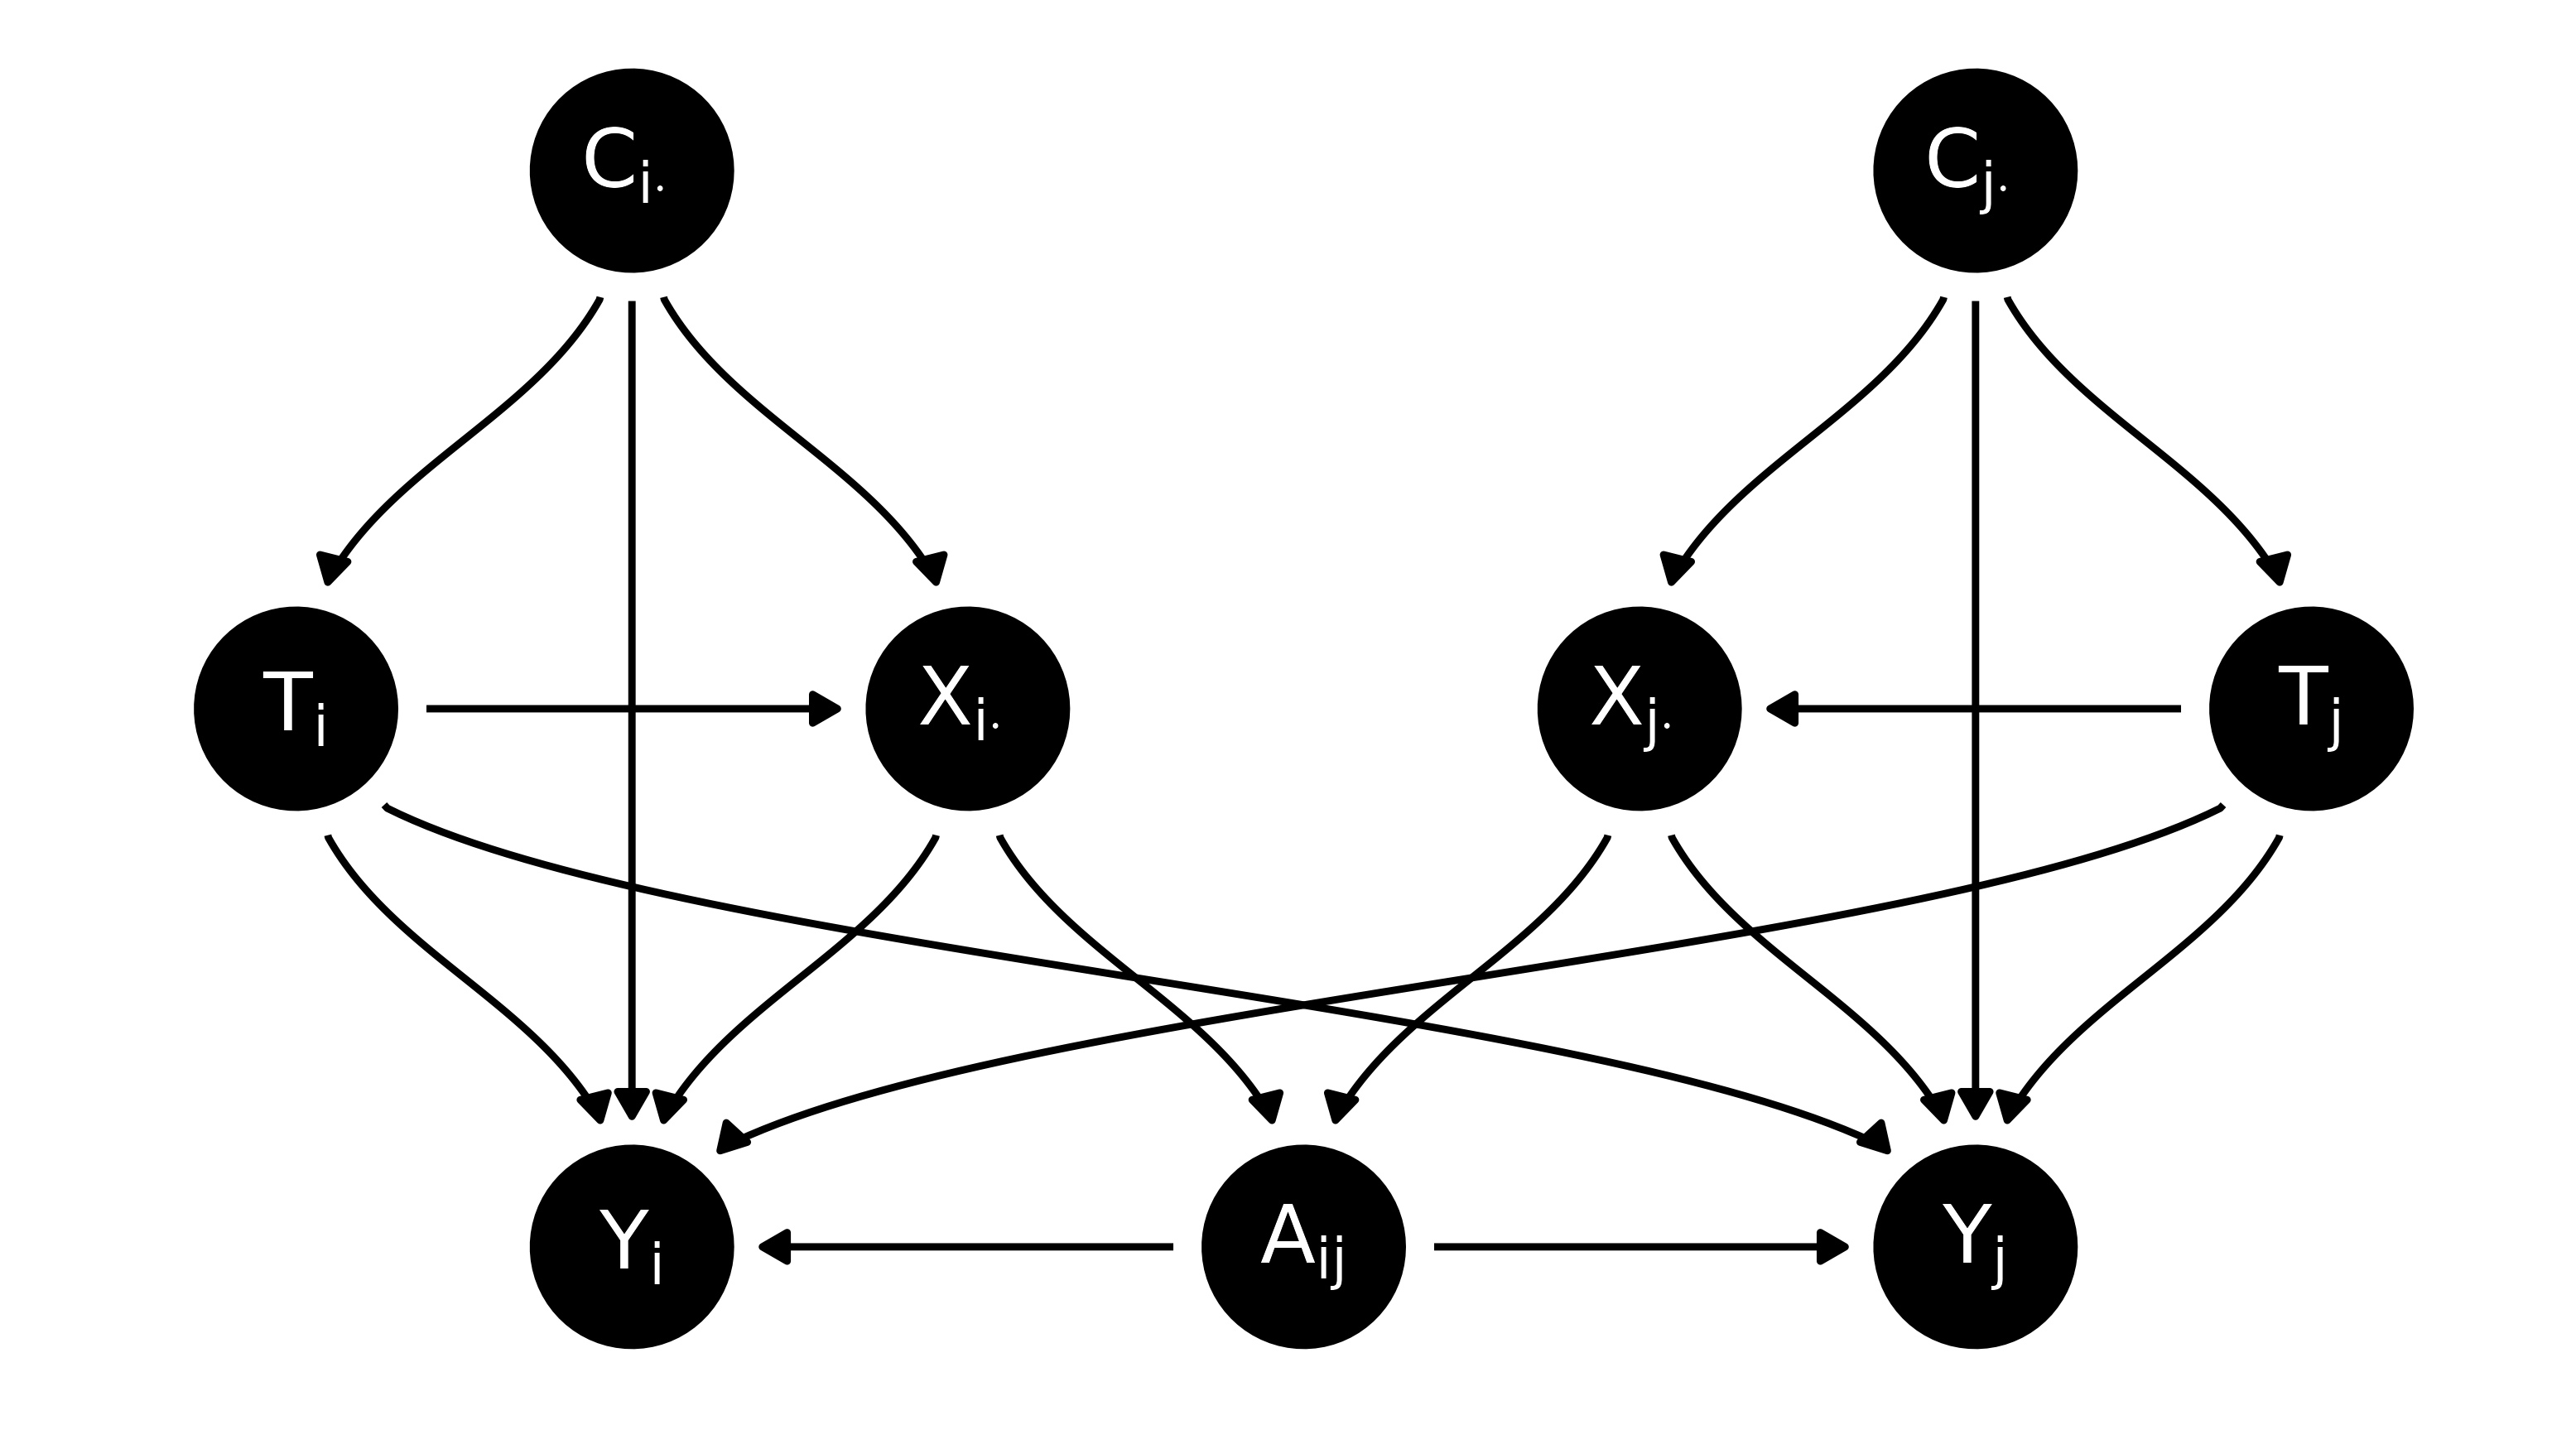
\includegraphics[scale=0.65]{figures/dags/interference.png}
        \label{fig:interference}
    \end{figure}

    Interference ($T_j \to Y_i$) is not allowed

\end{frame}

\begin{frame}{More on interference and contagion}

    Interference and contagion effects are allowed \emph{so long as they happen in the latent space}. Suppose
    \begin{align*}
        \E[\W_{i \cdot}, \X_{i \cdot}]{Y_i}
        = \W_{i \cdot} \betaw + \X_{i \cdot} \beta'_\text{x} + \delta_\text{y} \sum_{j} \X_{i \cdot}^T \X_{j \cdot} Y_j
    \end{align*}
    This latent space contagion model is a special parametric case of the regression outcome model (take $\betax = \beta'_\text{x} + \X^T Y \delta_\text{y}$).

\end{frame}

\begin{frame}{Semi-parametric network model}
    Let $A \in \R^{n \times n}$ be a random symmetric matrix, such as the adjacency matrix of an undirected graph. Let $\Apop = \E[\X]{A} = \X \X^T$ be the expectation of $A$ conditional on $\X \in \R^{n \times d}$, which has independent and identically distributed rows $\X_{1 \cdot}, \dots, \X_{n \cdot}$. That is, $\Apop$ has $\rank \paren*{\Apop} = d$ and is positive semi-definite with eigenvalues $\lambda_1 \ge \lambda_2 \ge \cdots \ge \lambda_d > 0 = \lambda_{d+1} = \cdots = \lambda_n$. Conditional on $\X$, the upper-triangular elements of $A - \Apop$ are independent $(\nu_n, b_n)$-sub-gamma random variables.
\end{frame}


\begin{frame}{Semi-parametric network model: identification of $\X$}

    $\Apop = \X \X^T = (\X Q) (\X Q)^T$ for any $d \times d$ orthogonal matrix $Q$, the latent positions $\X$ are only identifiable up to an orthogonal transformation.
\end{frame}

\begin{frame}{Choosing $\widehat{d}$: do a multiverse analysis}

    \centering

    \begin{figure}
        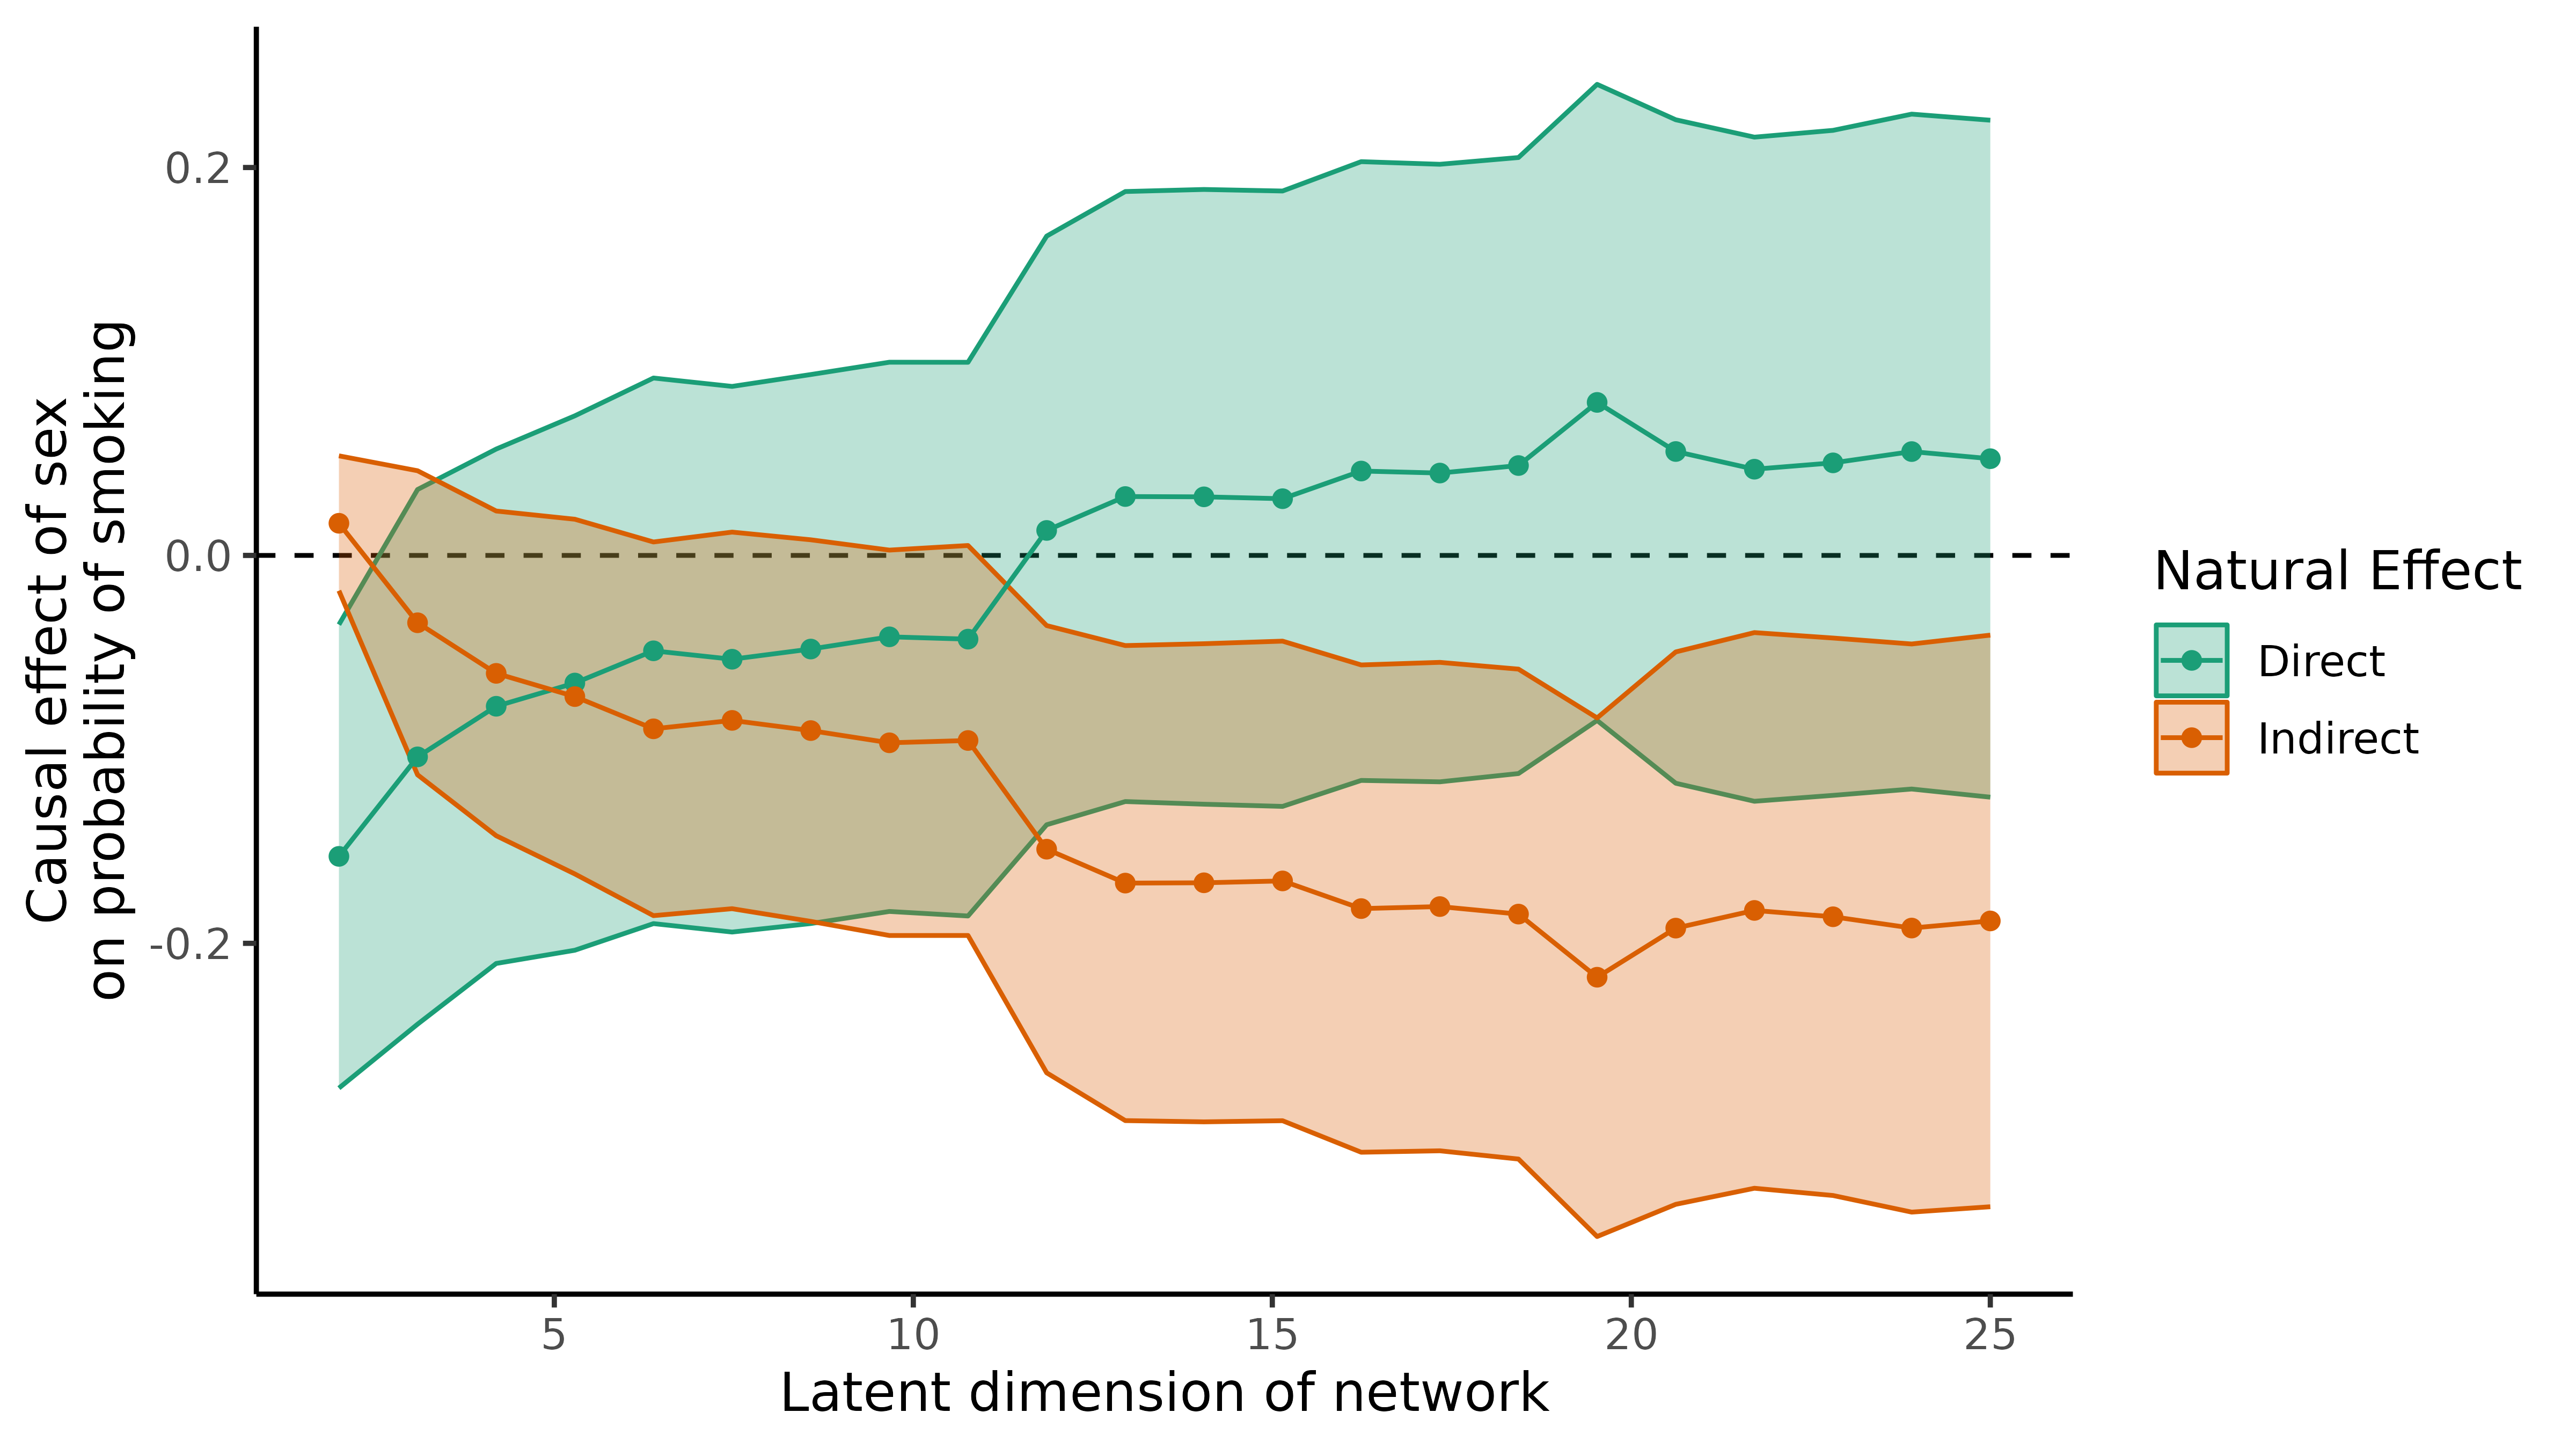
\includegraphics[width=\textwidth]{figures/glasgow-effects.png}
    \end{figure}

\end{frame}

\begin{frame}{Choosing $\widehat{d}$: overestimating the embedding dimension is fine}

    \centering

    \begin{figure}
        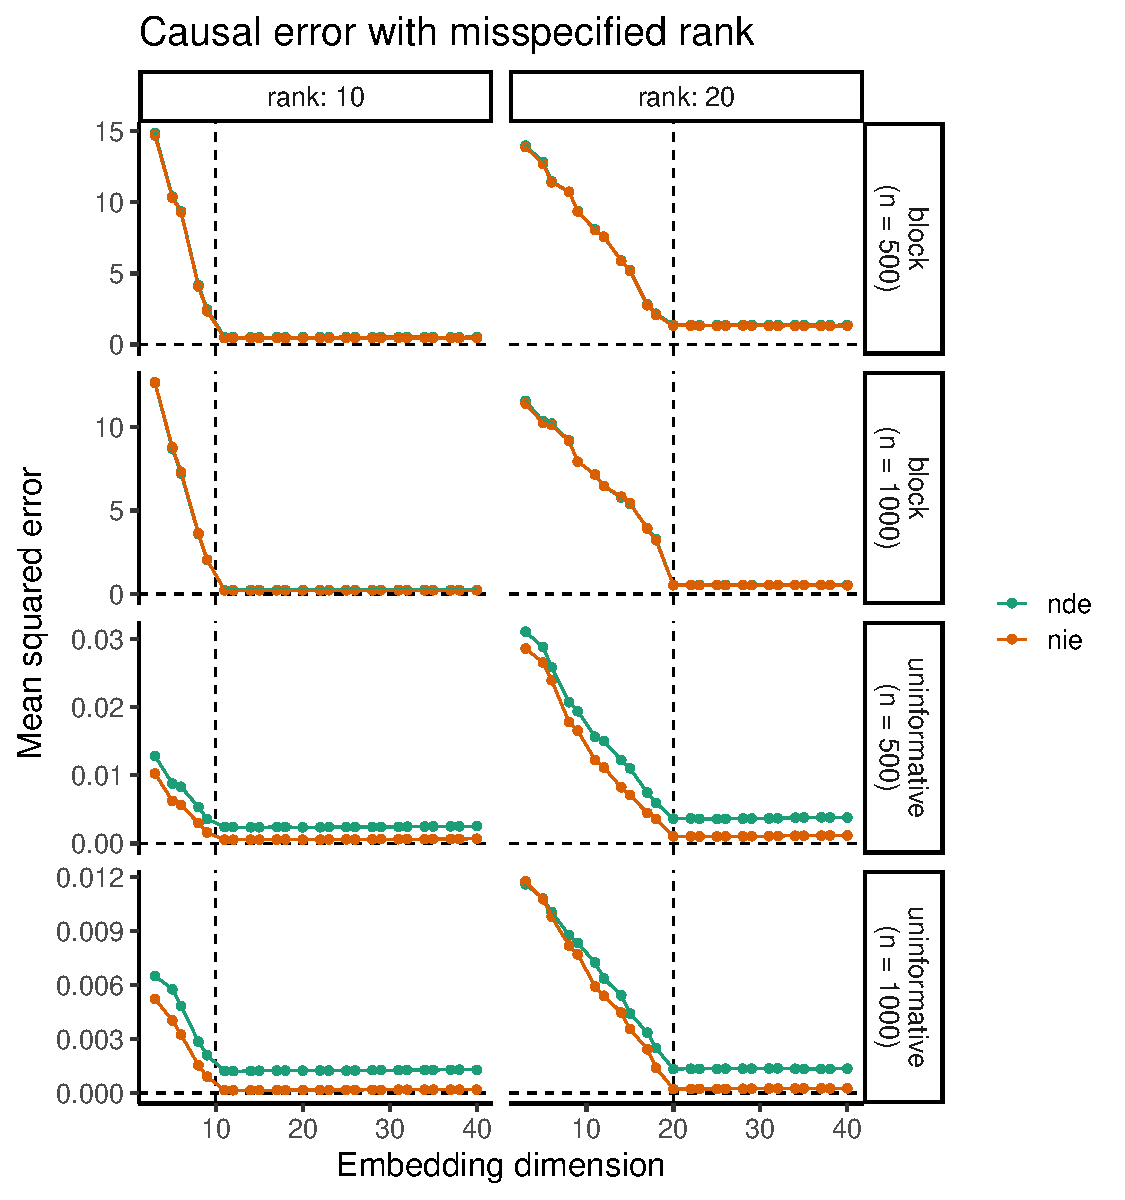
\includegraphics[width=0.7\textwidth]{figures/misspecification/loss_average.pdf}
    \end{figure}

\end{frame}

\begin{frame}{Identifying assumptions}

    The random variables $(Y_i, Y_i(t, x), \X_{i \cdot}, \X_{i \cdot}(t), C_{i \cdot}, T_i)$ are independent over $i \in [n]$ and obey the following three properties.
    \begin{enumerate}
        \item Consistency: \vspace{-3mm}
              \begin{equation*} \begin{aligned}
                       & \text{if $T_i = t$, then $\X_{i \cdot}(t) = \X_{i \cdot}$ with probability 1, and}    \\
                       & \text{if $T_i = t$ and $\X_{i \cdot} = x$, then $Y_i(t, x) = Y_i$ with probability 1}
                      \vspace{-2mm}
                  \end{aligned} \end{equation*}
        \item Sequential ignorability:
              \begin{equation*}
                  \set{Y_i(t^*, x), \X_{i \cdot}(t)} \indep T_i \cond \C_{i \cdot}
                  ~~~\text{ and }~~~
                  \set{Y_i(t^*, x)} \indep \X_{i \cdot}  \cond T_i = t, \C_{i \cdot}
              \end{equation*}
        \item Positivity:
              \begin{equation*}
                  \begin{aligned}
                      \P[T_i, \C_{i \cdot}]{x} & > 0 \text{ for each }  x \in \supp(\X_{i \cdot}) \\
                      \P[\C_{i \cdot}]{t}      & > 0 \text{ for each }  t \in \supp(T_i)
                  \end{aligned}
              \end{equation*}
    \end{enumerate}

\end{frame}

% \begin{frame}{Interventions on a network}

%     \begin{figure}
%         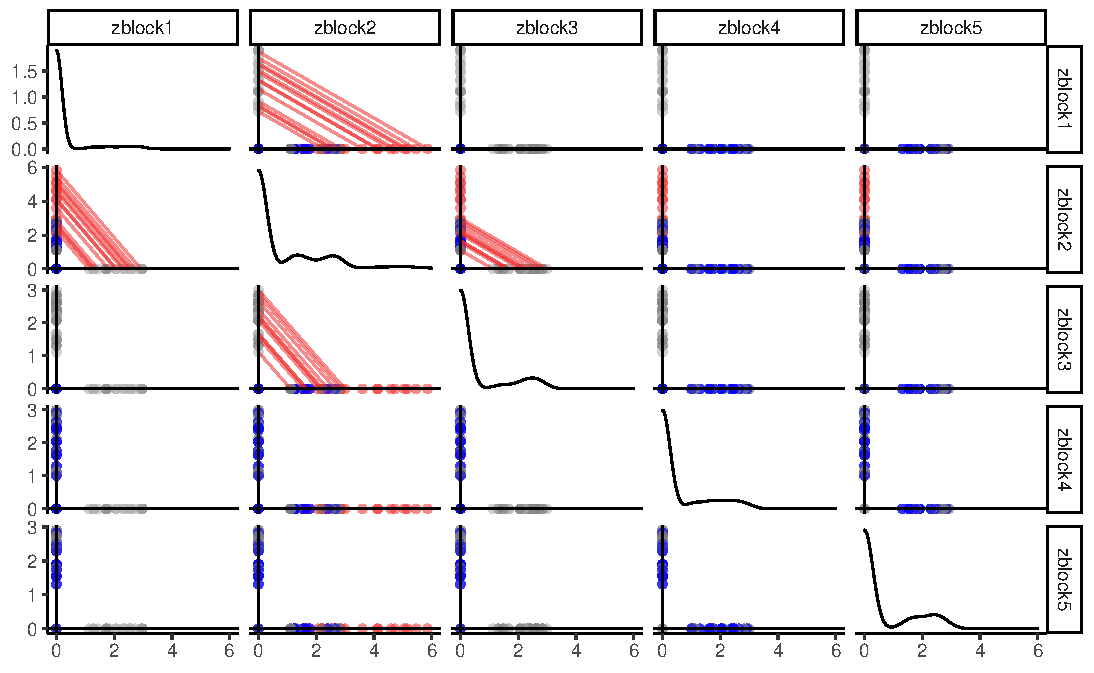
\includegraphics[width=\textwidth]{figures/intervention.pdf}
%         \caption{Canonical intervention when $\C$ is highly informative.}
%         \label{fig:intervention}
%     \end{figure}
% \end{frame}

% \begin{frame}{Interventions on a network}

%     \begin{align*}
%         \underbrace{\E[T_i, \C_{i \cdot}]{\Z_{i \cdot}}}_{\R^{1 \times d}}
%          & = \underbrace{\thetazero}_{\R^{1 \times d}}
%         + \underbrace{T_i}_{\{0, 1\}} \underbrace{\thetat}_{\R^{1 \times d}}
%         + \underbrace{\C_{i \cdot}}_{\R^{1 \times p}} \underbrace{\Thetac}_{\R^{p \times d}}
%         + \underbrace{T_i}_{\{0, 1\}} \underbrace{\C_{i \cdot}}_{\R^{1 \times p}} \underbrace{\Thetatc}_{\R^{p \times d}}.
%     \end{align*}

%     In Figure \ref{fig:intervention}, $\C$ are latent parameters for a DC-SBM and $\thetazero = \vec 0, \thetat = \vec 0, \Thetac = I_k$ and

%     \begin{align*}
%         \Thetatc =
%         \begin{bmatrix}
%             -1 & 2 & 0  & 0 & 0 \\
%             0  & 0 & 0  & 0 & 0 \\
%             0  & 1 & -1 & 0 & 0 \\
%             0  & 0 & 0  & 0 & 0 \\
%             0  & 0 & 0  & 0 & 0 \\
%         \end{bmatrix}
%     \end{align*}
% \end{frame}

\begin{frame}{Interventions allowed}

    Provided that controls $\C_{i \cdot}$ are sufficiently informative about group membership $\X_{i \cdot}$, treatment $T_i$ is allowed to cause:

    \begin{itemize}
        \item Changes in popularity within a group
        \item Movement to a new friend group
        \item Becoming a member of a new friend group while remaining in current friend group
        \item Friendships becoming more or less likely between distinct friend groups
        \item Combinations of the above
    \end{itemize}

    See Appendix of manuscript for details.

\end{frame}

\begin{frame}
    Emoji graphics licensed under CC-BY 4.0: https://creativecommons.org/licenses/by/4.0/
    Copyright 2019 Twitter, Inc and other contributors
\end{frame}

\bibliographystyle{chicago}
\bibliography{references}

\end{document}